%%%%%%%%%%%%%%%%%%%%%%%%%%%%%%%%%%%%%%%%%
% The Legrand Orange Book
% LaTeX Template
% Version 2.3 (8/8/17)
%
% This template has been downloaded from:
% http://www.LaTeXTemplates.com
%
% Original author:
% Mathias Legrand (legrand.mathias@gmail.com) with modifications by:
% Vel (vel@latextemplates.com)
%
% License:
% CC BY-NC-SA 3.0 (http://creativecommons.org/licenses/by-nc-sa/3.0/)
%
% Compiling this template:
% This template uses biber for its bibliography and makeindex for its index.
% When you first open the template, compile it from the command line with the 
% commands below to make sure your LaTeX distribution is configured correctly:
%
% 1) pdflatex main
% 2) makeindex main.idx -s StyleInd.ist
% 3) biber main
% 4) pdflatex main x 2
%
% After this, when you wish to update the bibliography/index use the appropriate
% command above and make sure to compile with pdflatex several times 
% afterwards to propagate your changes to the document.
%
% This template also uses a number of packages which may need to be
% updated to the newest versions for the template to compile. It is strongly
% recommended you update your LaTeX distribution if you have any
% compilation errors.
%
% Important note:
% Chapter heading images should have a 2:1 width:height ratio,
% e.g. 920px width and 460px height.
%
%%%%%%%%%%%%%%%%%%%%%%%%%%%%%%%%%%%%%%%%%

%----------------------------------------------------------------------------------------
%	PACKAGES AND OTHER DOCUMENT CONFIGURATIONS
%----------------------------------------------------------------------------------------

\documentclass[11pt,fleqn]{book} % Default font size and left-justified equations

%----------------------------------------------------------------------------------------

\usepackage[T1]{fontenc}
\usepackage{lmodern}

%%%%%%%%%%%%%%%%%%%%%%%%%%%%%%%%%%%%%%%%%
% The Legrand Orange Book
% Structural Definitions File
% Version 2.0 (9/2/15)
%
% Original author:
% Mathias Legrand (legrand.mathias@gmail.com) with modifications by:
% Vel (vel@latextemplates.com)
% 
% This file has been downloaded from:
% http://www.LaTeXTemplates.com
%
% License:
% CC BY-NC-SA 3.0 (http://creativecommons.org/licenses/by-nc-sa/3.0/)
%
%%%%%%%%%%%%%%%%%%%%%%%%%%%%%%%%%%%%%%%%%

%----------------------------------------------------------------------------------------
%	FONTS
%----------------------------------------------------------------------------------------

\usepackage{avant} % Use the Avantgarde font for headings
%\usepackage{times} % Use the Times font for headings
\usepackage{mathptmx} % Use the Adobe Times Roman as the default text font together with math symbols from the Sym­bol, Chancery and Com­puter Modern fonts

\usepackage{microtype} % Slightly tweak font spacing for aesthetics
\usepackage[utf8]{inputenc} % Required for including letters with accents
\usepackage[T1]{fontenc} % Use 8-bit encoding that has 256 glyphs
\setlength{\parskip}{0.2em} % paragraph spacing

%----------------------------------------------------------------------------------------
%	VARIOUS REQUIRED PACKAGES AND CONFIGURATIONS
%----------------------------------------------------------------------------------------

\usepackage[top=3cm,bottom=3cm,left=3cm,right=3cm,headsep=10pt,a4paper]{geometry} % Page margins

\usepackage{graphicx} % Required for including pictures
\graphicspath{{Pictures/}} % Specifies the directory where pictures are stored

%\usepackage{lipsum} % Inserts dummy text

\usepackage{tikz} % Required for drawing custom shapes

\usepackage[english]{babel} % English language/hyphenation
\usepackage{csquotes} % To allow quoted texts to follow same rules

\usepackage{enumitem} % Customize lists
\setlist{nolistsep} % Reduce spacing between bullet points and numbered lists

\usepackage{booktabs} % Required for nicer horizontal rules in tables
\usepackage{array} % Multiline in cells

\usepackage{xcolor} % Required for specifying colors by name
%\definecolor{basecolor}{RGB}{243,102,25} % Define the orange color used for highlighting throughout the book
\definecolor{basecolor}{RGB}{243,158,0} % Define the orange color used for highlighting throughout the book
%\definecolor{basecolor}{RGB}{255,191,0} % Define the base color used for highlighting throughout the book

\usepackage{float}
\restylefloat{table}

%----------------------------------------------------------------------------------------
%	BIBLIOGRAPHY AND INDEX
%----------------------------------------------------------------------------------------

\usepackage[style=numeric,citestyle=numeric,sorting=none,sortcites=true,autopunct=true,autolang=hyphen,hyperref=true,abbreviate=false,backref=true,backend=biber, maxbibnames=99]{biblatex}
\addbibresource{bibliography.bib} % BibTeX bibliography file
\defbibheading{bibempty}{}

\usepackage{calc} % For simpler calculation - used for spacing the index letter headings correctly
\usepackage{makeidx} % Required to make an index
\makeindex % Tells LaTeX to create the files required for indexing

%----------------------------------------------------------------------------------------
%	MAIN TABLE OF CONTENTS
%----------------------------------------------------------------------------------------

\usepackage{titletoc} % Required for manipulating the table of contents

\contentsmargin{0cm} % Removes the default margin

% Part text styling
\titlecontents{part}[0cm]
{\addvspace{20pt}\centering\large\bfseries}
{}
{}
{}

% Chapter text styling
\titlecontents{chapter}[1.25cm] % Indentation
{\addvspace{12pt}\large\sffamily\bfseries} % Spacing and font options for chapters
{\color{basecolor!60}\contentslabel[\Large\thecontentslabel]{1.25cm}\color{basecolor}} % Chapter number
{\color{basecolor}}  
{\color{basecolor!60}\normalsize\;\titlerule*[.5pc]{.}\;\thecontentspage} % Page number

% Section text styling
\titlecontents{section}[1.25cm] % Indentation
{\addvspace{3pt}\sffamily\bfseries} % Spacing and font options for sections
{\contentslabel[\thecontentslabel]{1.25cm}} % Section number
{}
{\hfill\color{black}\thecontentspage} % Page number
[]

% Subsection text styling
\titlecontents{subsection}[1.25cm] % Indentation
{\addvspace{1pt}\sffamily\small} % Spacing and font options for subsections
{\contentslabel[\thecontentslabel]{1.25cm}} % Subsection number
{}
{\ \titlerule*[.5pc]{.}\;\thecontentspage} % Page number
[]

% List of figures
\titlecontents{figure}[0em]
{\addvspace{-5pt}\sffamily}
{\thecontentslabel\hspace*{1em}}
{}
{\ \titlerule*[.5pc]{.}\;\thecontentspage}
[]

% List of tables
\titlecontents{table}[0em]
{\addvspace{-5pt}\sffamily}
{\thecontentslabel\hspace*{1em}}
{}
{\ \titlerule*[.5pc]{.}\;\thecontentspage}
[]

%----------------------------------------------------------------------------------------
%	MINI TABLE OF CONTENTS IN PART HEADS
%----------------------------------------------------------------------------------------

% Chapter text styling
\titlecontents{lchapter}[0em] % Indenting
{\addvspace{15pt}\large\sffamily\bfseries} % Spacing and font options for chapters
{\color{basecolor}\contentslabel[\Large\thecontentslabel]{1.25cm}\color{basecolor}} % Chapter number
{}  
{\color{basecolor}\normalsize\sffamily\bfseries\;\titlerule*[.5pc]{.}\;\thecontentspage} % Page number

% Section text styling
\titlecontents{lsection}[0em] % Indenting
{\sffamily\small} % Spacing and font options for sections
{\contentslabel[\thecontentslabel]{1.25cm}} % Section number
{}
{}

% Subsection text styling
\titlecontents{lsubsection}[.5em] % Indentation
{\normalfont\footnotesize\sffamily} % Font settings
{}
{}
{}

%----------------------------------------------------------------------------------------
%	PAGE HEADERS
%----------------------------------------------------------------------------------------

\usepackage{fancyhdr} % Required for header and footer configuration

\pagestyle{fancy}
\renewcommand{\chaptermark}[1]{\markboth{\sffamily\normalsize\bfseries\chaptername\ \thechapter.\ #1}{}} % Chapter text font settings
\renewcommand{\sectionmark}[1]{\markright{\sffamily\normalsize\thesection\hspace{5pt}#1}{}} % Section text font settings
\fancyhf{} \fancyhead[LE,RO]{\sffamily\normalsize\thepage} % Font setting for the page number in the header
\fancyhead[LO]{\rightmark} % Print the nearest section name on the left side of odd pages
\fancyhead[RE]{\leftmark} % Print the current chapter name on the right side of even pages
\renewcommand{\headrulewidth}{0.5pt} % Width of the rule under the header
\addtolength{\headheight}{2.5pt} % Increase the spacing around the header slightly
\renewcommand{\footrulewidth}{0pt} % Removes the rule in the footer
\fancypagestyle{plain}{\fancyhead{}\renewcommand{\headrulewidth}{0pt}} % Style for when a plain pagestyle is specified

% Removes the header from odd empty pages at the end of chapters
\makeatletter
\renewcommand{\cleardoublepage}{
\clearpage\ifodd\c@page\else
\hbox{}
\vspace*{\fill}
\thispagestyle{empty}
\newpage
\fi}

%----------------------------------------------------------------------------------------
%	THEOREM STYLES
%----------------------------------------------------------------------------------------

\usepackage{amsmath,amsfonts,amssymb,amsthm} % For math equations, theorems, symbols, etc

\newcommand{\intoo}[2]{\mathopen{]}#1\,;#2\mathclose{[}}
\newcommand{\ud}{\mathop{\mathrm{{}d}}\mathopen{}}
\newcommand{\intff}[2]{\mathopen{[}#1\,;#2\mathclose{]}}

\newtheorem{notation}{Notation}[chapter]
% Boxed/framed environments
\newtheoremstyle{mybasecolornumbox}% % Theorem style name
{0pt}% Space above
{0pt}% Space below
{\normalfont}% % Body font
{}% Indent amount
{\small\bf\sffamily\color{basecolor}}% % Theorem head font
{\;}% Punctuation after theorem head
{0.25em}% Space after theorem head
{\small\sffamily\color{basecolor}\thmname{#2}\nobreakspace\thmnumber{\@ifnotempty{#2}{}\@upn{#2}}% Theorem text (e.g. Theorem 2.1)
\thmnote{\nobreakspace\the\thm@notefont\sffamily\bfseries\color{black}---\nobreakspace#3.}} % Optional theorem note
\renewcommand{\qedsymbol}{$\blacksquare$}% Optional qed square

% Boxed/framed environments
\newtheoremstyle{basecolornumbox}% % Theorem style name
{0pt}% Space above
{0pt}% Space below
{\normalfont}% % Body font
{}% Indent amount
{\small\bf\sffamily\color{basecolor}}% % Theorem head font
{\;}% Punctuation after theorem head
{0.25em}% Space after theorem head
{\small\sffamily\color{basecolor}\thmname{#1}\nobreakspace\thmnumber{\@ifnotempty{#1}{}\@upn{#2}}% Theorem text (e.g. Theorem 2.1)
\thmnote{\nobreakspace\the\thm@notefont\sffamily\bfseries\color{black}---\nobreakspace#3.}} % Optional theorem note
\renewcommand{\qedsymbol}{$\blacksquare$}% Optional qed square

\newtheoremstyle{blacknumex}% Theorem style name
{5pt}% Space above
{5pt}% Space below
{\normalfont}% Body font
{} % Indent amount
{\small\bf\sffamily}% Theorem head font
{\;}% Punctuation after theorem head
{0.25em}% Space after theorem head
{\small\sffamily{\tiny\ensuremath{\blacksquare}}\nobreakspace\thmname{#1}\nobreakspace\thmnumber{\@ifnotempty{#1}{}\@upn{#2}}% Theorem text (e.g. Theorem 2.1)
\thmnote{\nobreakspace\the\thm@notefont\sffamily\bfseries---\nobreakspace#3.}}% Optional theorem note

\newtheoremstyle{blacknumbox} % Theorem style name
{0pt}% Space above
{0pt}% Space below
{\normalfont}% Body font
{}% Indent amount
{\small\bf\sffamily}% Theorem head font
{\;}% Punctuation after theorem head
{0.25em}% Space after theorem head
{\small\sffamily\thmname{#1}\nobreakspace\thmnumber{\@ifnotempty{#1}{}\@upn{#2}}% Theorem text (e.g. Theorem 2.1)
\thmnote{\nobreakspace\the\thm@notefont\sffamily\bfseries---\nobreakspace#3.}}% Optional theorem note

% Non-boxed/non-framed environments
\newtheoremstyle{basecolornum}% % Theorem style name
{5pt}% Space above
{5pt}% Space below
{\normalfont}% % Body font
{}% Indent amount
{\small\bf\sffamily\color{basecolor}}% % Theorem head font
{\;}% Punctuation after theorem head
{0.25em}% Space after theorem head
{\small\sffamily\color{basecolor}\thmname{#1}\nobreakspace\thmnumber{\@ifnotempty{#1}{}\@upn{#2}}% Theorem text (e.g. Theorem 2.1)
\thmnote{\nobreakspace\the\thm@notefont\sffamily\bfseries\color{black}---\nobreakspace#3.}} % Optional theorem note
\renewcommand{\qedsymbol}{$\blacksquare$}% Optional qed square
\makeatother

% Defines the theorem text style for each type of theorem to one of the three styles above
\newcounter{dummy} 
\numberwithin{dummy}{section}

\theoremstyle{basecolornumbox}
\newtheorem{theoremeT}[dummy]{Theorem}
\newtheorem{problem}{Problem}[chapter]
\newtheorem{exerciseT}{Exercise}[chapter]
\theoremstyle{blacknumex}
\newtheorem{exampleT}{Example}[chapter]
\theoremstyle{blacknumbox}
\newtheorem{vocabulary}{Vocabulary}[chapter]
\newtheorem{definitionT}{Definition}[section]
\newtheorem{corollaryT}[dummy]{Corollary}
\theoremstyle{basecolornum}
\newtheorem{proposition}[dummy]{Proposition}

%----------------------------------------------------------------------------------------
%	DEFINITION OF COLORED BOXES
%----------------------------------------------------------------------------------------

\RequirePackage[framemethod=default]{mdframed} % Required for creating the theorem, definition, exercise and corollary boxes

% Theorem box
\newmdenv[skipabove=7pt,
skipbelow=7pt,
backgroundcolor=black!5,
linecolor=basecolor,
innerleftmargin=5pt,
innerrightmargin=5pt,
innertopmargin=5pt,
leftmargin=0cm,
rightmargin=0cm,
innerbottommargin=2pt]{tBox}

% Exercise box	  
\newmdenv[skipabove=7pt,
skipbelow=7pt,
rightline=false,
leftline=true,
topline=false,
bottomline=false,
backgroundcolor=basecolor!10,
linecolor=basecolor,
innerleftmargin=5pt,
innerrightmargin=5pt,
innertopmargin=5pt,
innerbottommargin=5pt,
leftmargin=0cm,
rightmargin=0cm,
linewidth=4pt]{eBox}	

% Definition box
\newmdenv[skipabove=20pt,
skipbelow=7pt,
rightline=false,
leftline=true,
topline=false,
bottomline=false,
linecolor=basecolor,
innerleftmargin=5pt,
innerrightmargin=5pt,
innertopmargin=0pt,
leftmargin=0cm,
rightmargin=0cm,
linewidth=4pt,
innerbottommargin=0pt]{dBox}	

% Corollary box
\newmdenv[skipabove=7pt,
skipbelow=7pt,
rightline=false,
leftline=true,
topline=false,
bottomline=false,
linecolor=gray,
backgroundcolor=black!5,
innerleftmargin=5pt,
innerrightmargin=5pt,
innertopmargin=5pt,
leftmargin=0cm,
rightmargin=0cm,
linewidth=4pt,
innerbottommargin=5pt]{cBox}

% Creates an environment for each type of theorem and assigns it a theorem text style from the "Theorem Styles" section above and a colored box from above

\newenvironment{theorem}{\begin{tBox}\begin{theoremeT}}{\end{theoremeT}\end{tBox}}
\newenvironment{exercise}{\begin{eBox}\begin{exerciseT}}{\hfill{\color{basecolor}\tiny\ensuremath{\blacksquare}}\end{exerciseT}\end{eBox}}
\newenvironment{definition}{\begin{dBox}\begin{definitionT}}{\end{definitionT}\end{dBox}}
\newenvironment{example}{\begin{exampleT}}{\hfill{\tiny\ensuremath{\blacksquare}}\end{exampleT}}
\newenvironment{corollary}{\begin{cBox}\begin{corollaryT}}{\end{corollaryT}\end{cBox}}

%----------------------------------------------------------------------------------------
%	REMARK ENVIRONMENT
%----------------------------------------------------------------------------------------

\newenvironment{remark}{\par\vspace{10pt}\small % Vertical white space above the remark and smaller font size
\begin{list}{}{
\leftmargin=35pt % Indentation on the left
\rightmargin=25pt}\item\ignorespaces % Indentation on the right
\makebox[-2.5pt]{\begin{tikzpicture}[overlay]
\node[draw=basecolor!60,line width=1pt,circle,fill=basecolor!25,font=\sffamily\bfseries,inner sep=2pt,outer sep=0pt] at (-15pt,0pt){\textcolor{basecolor}{R}};\end{tikzpicture}} % Orange R in a circle
\advance\baselineskip -1pt}{\end{list}\vskip5pt} % Tighter line spacing and white space after remark

%----------------------------------------------------------------------------------------
%	SECTION NUMBERING IN THE MARGIN
%----------------------------------------------------------------------------------------

\makeatletter
\renewcommand{\@seccntformat}[1]{\llap{\textcolor{basecolor}{\csname the#1\endcsname}\hspace{1em}}}                    
\renewcommand{\section}{\@startsection{section}{1}{\z@}
{-4ex \@plus -1ex \@minus -.4ex}
{1ex \@plus.2ex }
{\normalfont\large\sffamily\bfseries}}
\renewcommand{\subsection}{\@startsection {subsection}{2}{\z@}
{-3ex \@plus -0.1ex \@minus -.4ex}
{0.5ex \@plus.2ex }
{\normalfont\sffamily\bfseries}}
\renewcommand{\subsubsection}{\@startsection {subsubsection}{3}{\z@}
{-2ex \@plus -0.1ex \@minus -.2ex}
{.2ex \@plus.2ex }
{\normalfont\small\sffamily\bfseries}}                        
\renewcommand\paragraph{\@startsection{paragraph}{4}{\z@}
{-2ex \@plus-.2ex \@minus .2ex}
{.1ex}
{\normalfont\small\sffamily\bfseries}}

%----------------------------------------------------------------------------------------
%	PART HEADINGS
%----------------------------------------------------------------------------------------

% numbered part in the table of contents
\newcommand{\@mypartnumtocformat}[2]{%
\setlength\fboxsep{0pt}%
\noindent\colorbox{basecolor!20}{\strut\parbox[c][.7cm]{\ecart}{\color{basecolor!70}\Large\sffamily\bfseries\centering#1}}\hskip\esp\colorbox{basecolor!40}{\strut\parbox[c][.7cm]{\linewidth-\ecart-\esp}{\Large\sffamily\centering#2}}}%
%%%%%%%%%%%%%%%%%%%%%%%%%%%%%%%%%%
% unnumbered part in the table of contents
\newcommand{\@myparttocformat}[1]{%
\setlength\fboxsep{0pt}%
\noindent\colorbox{basecolor!40}{\strut\parbox[c][.7cm]{\linewidth}{\Large\sffamily\centering#1}}}%
%%%%%%%%%%%%%%%%%%%%%%%%%%%%%%%%%%
\newlength\esp
\setlength\esp{4pt}
\newlength\ecart
\setlength\ecart{1.2cm-\esp}
\newcommand{\thepartimage}{}%
\newcommand{\partimage}[1]{\renewcommand{\thepartimage}{#1}}%
\def\@part[#1]#2{%
\ifnum \c@secnumdepth >-2\relax%
\refstepcounter{part}%
\addcontentsline{toc}{part}{\texorpdfstring{\protect\@mypartnumtocformat{\thepart}{#1}}{\partname~\thepart\ ---\ #1}}
\else%
\addcontentsline{toc}{part}{\texorpdfstring{\protect\@myparttocformat{#1}}{#1}}%
\fi%
\startcontents%
\markboth{}{}%
{\thispagestyle{empty}%
\begin{tikzpicture}[remember picture,overlay]%
\node at (current page.north west){\begin{tikzpicture}[remember picture,overlay]%	
\fill[basecolor!20](0cm,0cm) rectangle (\paperwidth,-\paperheight);
\node[anchor=north] at (4cm,-3.25cm){\color{basecolor!40}\fontsize{220}{100}\sffamily\bfseries\thepart}; 
\node[anchor=south east] at (\paperwidth-1cm,-\paperheight+1cm){\parbox[t][][t]{8.5cm}{
\printcontents{l}{0}{\setcounter{tocdepth}{1}}%
}};
\node[anchor=north east] at (\paperwidth-1.5cm,-3.25cm){\parbox[t][][t]{15cm}{\strut\raggedleft\color{white}\fontsize{30}{30}\sffamily\bfseries#2}};
\end{tikzpicture}};
\end{tikzpicture}}%
\@endpart}
\def\@spart#1{%
\startcontents%
\phantomsection
{\thispagestyle{empty}%
\begin{tikzpicture}[remember picture,overlay]%
\node at (current page.north west){\begin{tikzpicture}[remember picture,overlay]%	
\fill[basecolor!20](0cm,0cm) rectangle (\paperwidth,-\paperheight);
\node[anchor=north east] at (\paperwidth-1.5cm,-3.25cm){\parbox[t][][t]{15cm}{\strut\raggedleft\color{white}\fontsize{30}{30}\sffamily\bfseries#1}};
\end{tikzpicture}};
\end{tikzpicture}}
\addcontentsline{toc}{part}{\texorpdfstring{%
\setlength\fboxsep{0pt}%
\noindent\protect\colorbox{basecolor!40}{\strut\protect\parbox[c][.7cm]{\linewidth}{\Large\sffamily\protect\centering #1\quad\mbox{}}}}{#1}}%
\@endpart}
\def\@endpart{\vfil\newpage
\if@twoside
\if@openright
\null
\thispagestyle{empty}%
\newpage
\fi
\fi
\if@tempswa
\twocolumn
\fi}

%----------------------------------------------------------------------------------------
%	CHAPTER HEADINGS
%----------------------------------------------------------------------------------------

% A switch to conditionally include a picture, implemented by  Christian Hupfer
\newif\ifusechapterimage
\usechapterimagetrue
\newcommand{\thechapterimage}{}%
\newcommand{\chapterimage}[1]{\ifusechapterimage\renewcommand{\thechapterimage}{#1}\fi}%
\newcommand{\autodot}{.}
\def\@makechapterhead#1{%
{\parindent \z@ \raggedright \normalfont
\ifnum \c@secnumdepth >\m@ne
\if@mainmatter
\begin{tikzpicture}[remember picture,overlay]
\node at (current page.north west)
{\begin{tikzpicture}[remember picture,overlay]
\node[anchor=north west,inner sep=0pt] at (0,0) {\ifusechapterimage\includegraphics[width=\paperwidth]{\thechapterimage}\fi};
\draw[anchor=west] (\Gm@lmargin,-9cm) node [line width=2pt,rounded corners=15pt,draw=basecolor,fill=white,fill opacity=0.5,inner sep=15pt]{\strut\makebox[22cm]{}};
\draw[anchor=west] (\Gm@lmargin+.3cm,-9cm) node {\huge\sffamily\bfseries\color{black}\thechapter\autodot~#1\strut};
\end{tikzpicture}};
\end{tikzpicture}
\else
\begin{tikzpicture}[remember picture,overlay]
\node at (current page.north west)
{\begin{tikzpicture}[remember picture,overlay]
\node[anchor=north west,inner sep=0pt] at (0,0) {\ifusechapterimage\includegraphics[width=\paperwidth]{\thechapterimage}\fi};
\draw[anchor=west] (\Gm@lmargin,-9cm) node [line width=2pt,rounded corners=15pt,draw=basecolor,fill=white,fill opacity=0.5,inner sep=15pt]{\strut\makebox[22cm]{}};
\draw[anchor=west] (\Gm@lmargin+.3cm,-9cm) node {\huge\sffamily\bfseries\color{black}#1\strut};
\end{tikzpicture}};
\end{tikzpicture}
\fi\fi\par\vspace*{270\p@}}}

%-------------------------------------------

\def\@makeschapterhead#1{%
\begin{tikzpicture}[remember picture,overlay]
\node at (current page.north west)
{\begin{tikzpicture}[remember picture,overlay]
\node[anchor=north west,inner sep=0pt] at (0,0) {\ifusechapterimage\includegraphics[width=\paperwidth]{\thechapterimage}\fi};
\draw[anchor=west] (\Gm@lmargin,-9cm) node [line width=2pt,rounded corners=15pt,draw=basecolor,fill=white,fill opacity=0.5,inner sep=15pt]{\strut\makebox[22cm]{}};
\draw[anchor=west] (\Gm@lmargin+.3cm,-9cm) node {\huge\sffamily\bfseries\color{black}#1\strut};
\end{tikzpicture}};
\end{tikzpicture}
\par\vspace*{270\p@}}
\makeatother

%----------------------------------------------------------------------------------------
%	HYPERLINKS IN THE DOCUMENTS
%----------------------------------------------------------------------------------------

\usepackage{hyperref}
\hypersetup{hidelinks,colorlinks=false,breaklinks=true,urlcolor= basecolor,bookmarksopen=false,pdftitle={dataClay Manual}}
\usepackage{bookmark}
\bookmarksetup{
open,
numbered,
addtohook={%
\ifnum\bookmarkget{level}=0 % chapter
\bookmarksetup{bold}%
\fi
\ifnum\bookmarkget{level}=-1 % part
\bookmarksetup{color=basecolor,bold}%
\fi
}
}

%----------------------------------------------------------------------------------------
%	VERBATIM FOR CODE EXAMPLES
%----------------------------------------------------------------------------------------
\usepackage{fancyvrb}
\usepackage{listingsutf8}
\usepackage{color}

\definecolor{dkgreen}{rgb}{0,0.6,0}
\definecolor{gray}{rgb}{0.5,0.5,0.5}
\definecolor{mauve}{rgb}{0.58,0,0.82}

\newcommand\javastyle{\lstset{frame=none,
  language=Java,
  aboveskip=3mm,
  belowskip=3mm,
  showstringspaces=false,
  columns=flexible,
  basicstyle={\scriptsize\ttfamily},
  otherkeywords={this},            
  numbers=none,
  keywordstyle=\color{blue},
  commentstyle=\color{dkgreen},
  stringstyle=\color{mauve},
  breaklines=true,
  breakatwhitespace=true,
  tabsize=3
}}

% Java environment
\lstnewenvironment{java}[1][]
{
\javastyle
\lstset{#1}
}
{}

% Python for inline
\newcommand\javainline[1]{{\javastyle\lstinline!#1!}}

\newcommand\pythonstyle{\lstset{frame=none,
  language=Python,
  aboveskip=3mm,
  belowskip=3mm,
  showstringspaces=false,
  columns=flexible,
  basicstyle={\scriptsize\ttfamily},
  otherkeywords={self, dclayMethod},             % Add keywords here
  numbers=none,
  keywordstyle=\color{blue},
  commentstyle=\color{dkgreen},
  emph={MyClass,__init__},          % Custom highlighting
  emphstyle=\color{mauve},    % Custom highlighting style
  numberstyle=\tiny\color{gray},
  stringstyle=\color{mauve},
  breaklines=true,
  breakatwhitespace=true,
  tabsize=3
}}

% Python environment
\lstnewenvironment{python}[1][]
{
\pythonstyle
\lstset{#1}
}
{}

% Python for inline
\newcommand\pythoninline[1]{{\pythonstyle\lstinline!#1!}}

% Bash
\newcommand\bashstyle{\lstset{frame=none,
  language=bash,
  aboveskip=3mm,
  belowskip=3mm,
  showstringspaces=false,
  columns=flexible,
  basicstyle={\scriptsize\ttfamily},
  numbers=none,
  keywordstyle=\color{blue},
  commentstyle=\color{dkgreen},
  emphstyle=\color{mauve},    % Custom highlighting style
  numberstyle=\tiny\color{gray},
  stringstyle=\color{mauve},
  breaklines=true,
  breakatwhitespace=true,
  tabsize=3
}}

% Bash environment
\lstnewenvironment{bash}[1][]
{
\bashstyle
\lstset{#1}
}
{}

% Bash for inline
\newcommand\bashinline[1]{{\bashstyle\lstinline!#1!}}


% Docker
\lstdefinelanguage{docker-compose-2}{
  keywords={version, volumes, services},
  keywordstyle=\color{blue}\bfseries,
  keywords=[2]{image, environment, env\_file, volume, command, ports, container_name, ports, links, build, network\_mode},
  keywordstyle=[2]\color{olive}\bfseries,
  basicstyle={\scriptsize\ttfamily},
  identifierstyle=\color{black},
  sensitive=false,
  columns=flexible,
  comment=[l]{\#},
  commentstyle=\color{violet}\ttfamily,
  stringstyle=\ttfamily,
  morestring=[b]',
  morestring=[b]"
}
 % Insert the structure.tex file which contains the majority of the structure behind the template

\newcounter{todos}
\setcounter{todos}{0}
\newcommand{\TODO}[1]
{
\begin{eBox}\addtocounter{todos}{1}\textcolor{red}{\bf TODO [\arabic{todos}] -- }\textcolor{red}{#1}\end{eBox}
}

\newcounter{codetodos}
\setcounter{codetodos}{0}
\newcommand{\CODETODO}[1]
{
\begin{eBox}\addtocounter{codetodos}{1}\textcolor{green}{\bf CHANGE CODE [\arabic{codetodos}] -- }\textcolor{green}{#1}\end{eBox}
}

\newcounter{discusstodos}
\setcounter{discusstodos}{0}
\newcommand{\DISCUSS}[1]
{
\begin{eBox}\addtocounter{discusstodos}{1}\textcolor{blue}{\bf DISCUSS [\arabic{discusstodos}] -- }\textcolor{blue}{#1}\end{eBox}
}

\newcounter{checktodos}
\setcounter{checktodos}{0}
\newcommand{\CHECK}[1]
{
\begin{eBox}\addtocounter{checktodos}{1}\textcolor{orange}{\bf CHECK [\arabic{checktodos}] -- }\textcolor{orange}{#1}\end{eBox}
}

\newcommand{\CALL}[1]
{
{\bfseries\textcolor{basecolor}{#1}}\index{#1}
}

\newcommand{\LINE}{
\newline\rule{\textwidth}{0.4pt}
}

\newcommand{\FEDERATION}[1]
{
#1
}

\newcommand{\FILTERING}[1]
{
%#1
}

\newcommand{\PREFETCH}[1]
{
%#1
}

\begin{document}



%----------------------------------------------------------------------------------------
%	TITLE PAGE
%----------------------------------------------------------------------------------------

\begingroup
\thispagestyle{empty}
\begin{tikzpicture}[remember picture,overlay]
%\node[inner sep=0pt] (background) at (current page.center) {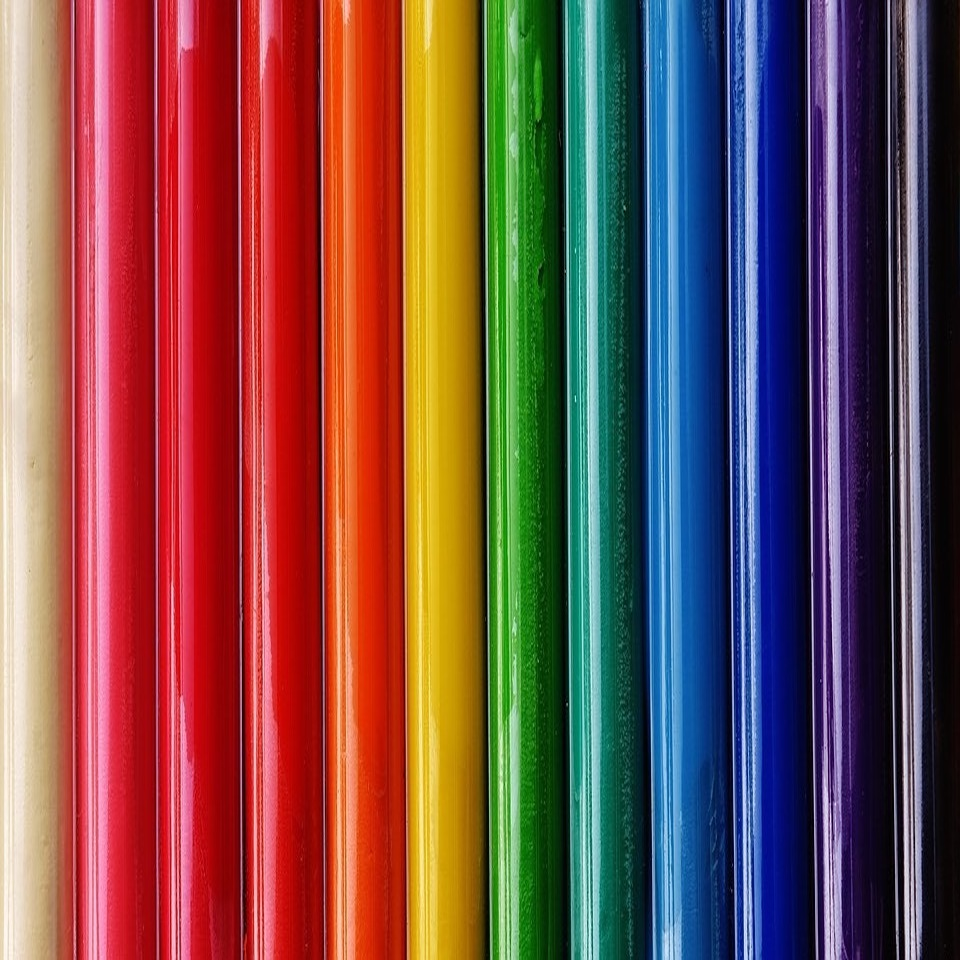
\includegraphics[width=\paperwidth]{background.jpg}};
\node[inner sep=0pt] (background) at (current page.north) {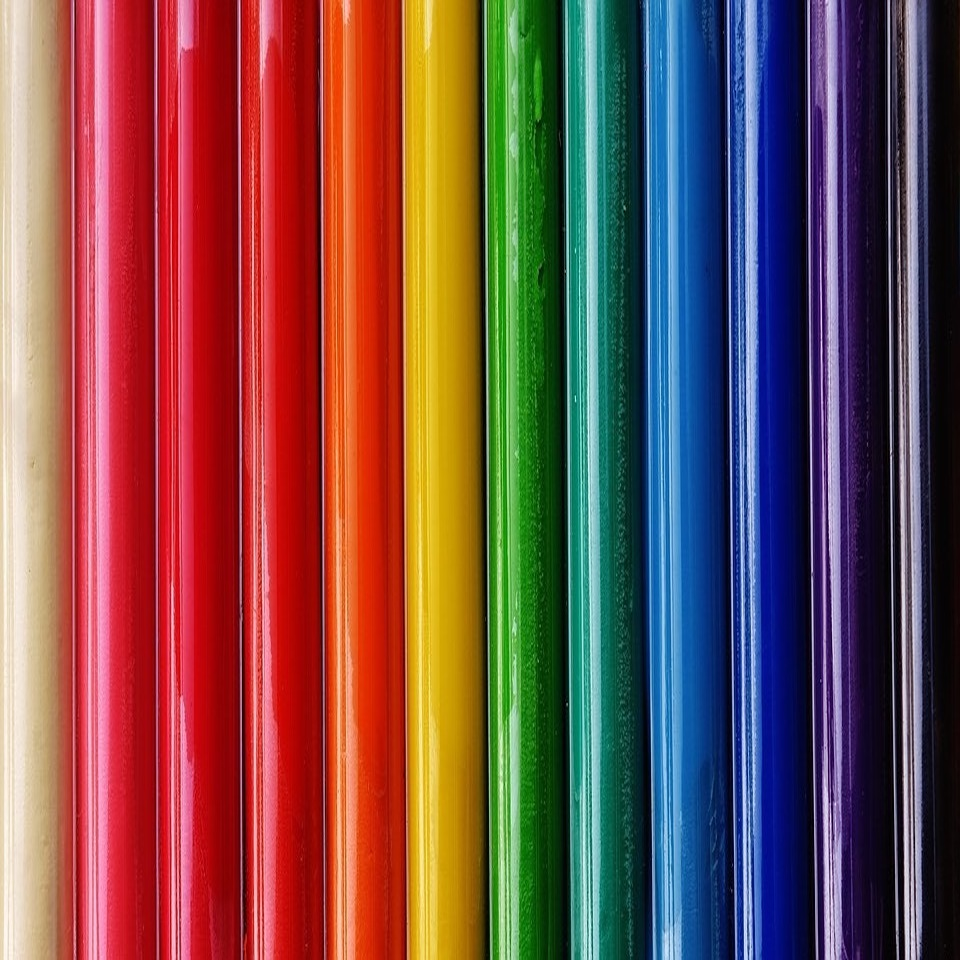
\includegraphics[width=\paperwidth]{background.jpg}};
\node[inner sep=0pt] (background) at (current page.south) {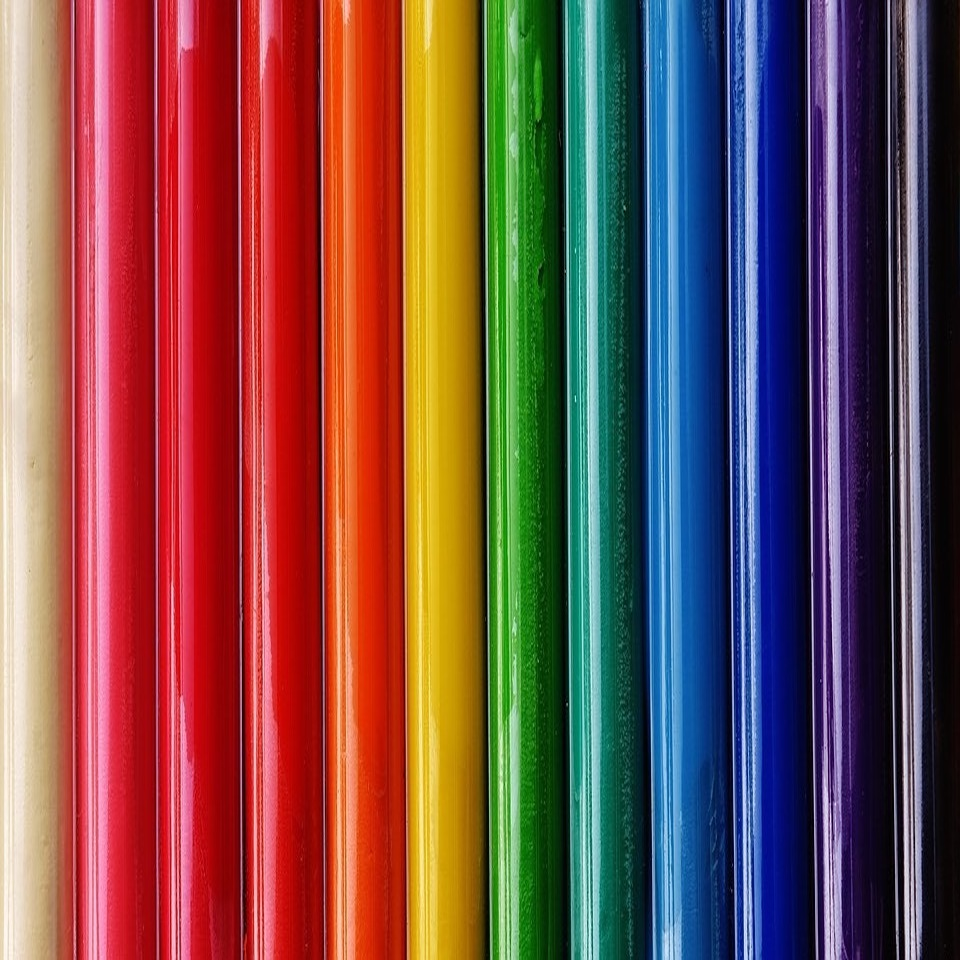
\includegraphics[width=\paperwidth]{background.jpg}};

\definecolor{mygray}{rgb}{0.40,0.40,0.40}

\draw (current page.center) node [fill=white,fill opacity=0.6,text opacity=1,inner sep=1cm]{\Huge\centering\bfseries\sffamily\parbox[c][][t]{\paperwidth}{\centering\color{mygray}  Manual\\[8pt] % Book title
%{\Large Manual}\\[20pt] % Subtitle

\centering
\includegraphics[width=8cm]{dClaylogo.jpg}

{\Large version 2.0}\\[10pt] % version
{\huge Barcelona Supercomputing Center}\\[8pt] % Author name
{\Large support-dataclay@bsc.es}}}; % Author email
\end{tikzpicture}
\vfill
\endgroup

%----------------------------------------------------------------------------------------
%	RELEASE NOTES
%----------------------------------------------------------------------------------------

\cleardoublepage % Forces the first chapter to start on an odd page so it's on the right

\chapterimage{TOC.jpg} % Chapter heading image
\chapter*{Release notes}

\begin{itemize}
\item[] \textbf{2020, June : Release version 2.4}\newline
    \begin{itemize}
    \item[] \textbf{New features}
        \begin{itemize}
            \item[] Support for Python 3.7 and 3.8
            \item[] Support for ARM 64-bit architecture
            \item[] Integrated Paraver tracing for applications using dataClay and COMPSs
        \end{itemize}
    \item[] \textbf{Improvements}
        \begin{itemize}
            \item[] Improved performance in \textit{get by alias}
            \item[] Improved Singularity deployment
            \item[] New deployable demos and updated examples
            \item[] Bug fixes
        \end{itemize}
    \end{itemize}
\end{itemize}


%----------------------------------------------------------------------------------------
%	TABLE OF CONTENTS
%----------------------------------------------------------------------------------------

%\usechapterimagefalse % If you don't want to include a chapter image, use this to toggle images off - it can be enabled later with \usechapterimagetrue

\chapterimage{TOC.jpg} % Table of contents heading image

\pagestyle{empty} % No headers

\tableofcontents % Print the table of contents itself

\cleardoublepage % Forces the first chapter to start on an odd page so it's on the right

\pagestyle{fancy} % Print headers again
\rhead{\begin{picture}(0,0) \put(-60,0){
\includegraphics[width=2cm]{dClaylogo.jpg}}\end{picture}}

\renewcommand\labelitemi{}
\setlength{\parindent}{0pt}


%----------------------------------------------------------------------------------------
%	PART
%----------------------------------------------------------------------------------------

\part{Getting started}
  \chapterimage{FirstSteps.jpg} % Chapter heading image

\chapter{Main Concepts}

\section{What is dataClay}

dataClay~\cite{MARTI2017129,MartiFraiz2017} is a distributed object store that enables programmers to handle object persistence using the same model they use in their object-oriented applications, thus avoiding time consuming transformation between persistent and non persistent models. In other words, dataClay enables applications to store objects in the same format they have in memory. This can be done either using the standard \textit{GET/PUT/UPDATE} methods of standard object stores, or by just calling the \textit{makePersistent} method on an object that will enable applications to access it, in the same way, regardless of whether it is loaded in memory or persisted in disk (you just follow the object reference).

In addition, dataClay simplifies and optimizes the idea of moving computation close to data (see Section~\ref{sec:ExecutionModel}) by enabling the execution of methods in the same node where a given object is located. dataClay also optimizes the idea of sharing data and models (set of classes) between different users by means of storing the class (including method definition) together with the object.

\section{Basic terminology}

In this section we present a brief terminology that is used throughout the manual. 

\begin{itemize}

\item {\bf Object}\index{object}, as in object oriented programming, refers to a particular instance of a class.

\item {\bf dataClay application}\index{dataClay application} is any application that uses dataClay to handle its persistent data. 

\item {\bf Backend}\index{backend} is a node in the system that is able to handle persistent objects and execution requests. These nodes need to be running the dataClay platform on them. We can have as many as we need either for capacity or parallelism reasons.

\item {\bf Clients}\index{client} are the machines where dataClay applications run. These nodes can be very thin. They only need to be able to run Java or Python code and to have the dataClay lib installed.

\item {\bf dataClay object}\index{dataClay object}\index{object} is any object stored in dataClay.

\item {\bf Objects with alias}\index{alias} are objects that have been explicitly named (much in the same way we give names to files). Not all dataClay objects need to have an alias (a name). If an object has an alias, we can access it by using its name. On the other hand, objects without an alias can only be accessed by a reference from another object. 

\item {\bf Dataset}\index{dataset} is an abstraction where many objects are grouped. It is indented to simplify the task of sharing objects with other users.

\item {\bf Data model}\index{data model} or \textbf{class model} consists of a set of related classes programmed in one of the supported languages (Java 11 or Python 3).

\item {\bf Namespace}\index{namespace}  is a dataClay abstraction aimed at grouping a set of classes together. Namespaces have two objectives: i) grouping related classes to ease the task of sharing them with other users and ii) avoiding clashing of class names. A namespace is similar to a Java/Python package.

\end{itemize}

\section{Execution model}
\label{sec:ExecutionModel}\index{execution model}

As we have mentioned, one of the key features of dataClay is to offer a mechanism to bring computation closer to data. For this reason, all methods of a dataClay object will not be executed in the client (application address space) but on the backend where dataClay stored the object. Thus, searching for an object in a collection will not imply sending all objects in the collection to the client, but only the final result because the search method will be executed in the backend. If the collection is distributed among different backends, any sub-method required to check whether objects match certain conditions or not, will be executed on the involved backends.

It is important to notice that this execution model does not prevent developers to use the standard object store model by using \textit{GET/PUT/UPDATE} methods. In particular, a \textit{GET} method (as \textit{CLONE} in dataClay to match with object oriented terminology), will bring the object to the application address space and thus all methods will be executed locally. At this point, any application object either retrieved (\textit{CLONED}) from dataClay or created by the application itself, can be either \textit{PUT} into the system to save it or can be used to \textit{UPDATE} an existing stored object.

\section{Tasks and roles}\index{roles}

In order to rationalize the different roles that take part in data-centric applications, such as the ones supported by dataClay, we assume two different roles.

\begin{itemize}

\item {\bf Model providers}\index{model provider} design and implement class models to define the elements of data (data structure), their relationships, and methods (API) that applications can use to access and process it.

\item {\bf Application developers}\index{application developer} use classes developed by the model provider in order to build applications. These applications can either create and store new objects or access data previously created.

\end{itemize}

Although dataClay encourages these roles in the cycle of applications, they do not have to be declared as such and, of course, they can be assumed by a single person.

\section{Memory Management and Garbage Collection}
\label{sec:GarbageCollection}\index{garbage collection}\index{memory management}

Every backend in dataClay maintains a daemon process that checks if memory usage has reached a certain threshold and, if this is the case, it flushes those objects that are not referenced into the underlying storage.

On the other hand, dataClay also performs background garbage collection to remove those objects that are no longer accessible. More specifically, dataClay deploys a distributed garbage collection service, involving all the backends, to periodically collect any object meeting the following conditions:
\begin{enumerate}
  \item The object is not pointed by any other object.
  \item The object has no aliases.
  \item There is no user application referencing the object.
  \item There is no backend accessing the object from a running execution method.
\end{enumerate}

\PREFETCH{
\section{Data Prefetching}
\label{sec:prefetching}\index{prefetching}
As a performance improvement mechanism, the user can choose to activate data prefetching in dataClay. When prefetching is activated, dataClay prefetches the data from the persistent storage of each backend into its main memory. There are two different types of prefetching:
\begin{enumerate}
    \item the default 'smart' prefetching based on code analysis of the applications.
    \item a lightweight alternative that prefetches objects referenced from a specific object when it is accessed.
\end{enumerate}
Choosing the desired type of prefetching can be done while registering a new model using dataClay tool, as explained in Section \ref{sec:newModel}. Note that once a model is registered with one type of prefetching, it cannot be changed later to use the other type.

The prefetching module is still experimental and in order for it to function properly, the client application must meet the following conditions:

\begin{enumerate}
    \item The application must be written in Java. Data prefetching is currently not available for Python applications.
    \item The application must contain one class definition per file.
    \item All collections defined in the application must be typed. If a collection is not typed, it will be ignored by the prefetching module.
    \item The application must not contain constructs specific to Java 1.8, such as lambda expressions or collection streams.
\end{enumerate}
}

\FEDERATION{
\section{Federation}
\label{sec:federation}\index{federation}
In some scenarios, such as edge-to-cloud deployments, part of the data stored in a dataClay instance has to be shared with another dataClay instance running in a different device. An example can be found in the context of smart cities where, for instance, part of the data residing in a car is temporarily shared with the city the car is traversing. This partial, and possibly temporal, integration of data between independent dataClay instances is implemented by means of dataClay's federation mechanism.
More precisely, federation consists in replicating an object (either simple or complex, such as a collection of objects) in an independent dataClay instance so that the recipient dataClay can access the object without the need to contact the owner dataClay. This provides immediate access to the object, avoiding communications when the object is requested and overcoming the possible unavailability of the data source. 
}
  \chapterimage{FirstSteps.jpg} % Chapter heading image

\chapter{My first dataClay application}
\label{sec:MyFirstApplication}

In order to better understand what dataClay is and how it is used, we present a very simple example (HelloPeople) where data is stored using dataClay. Sections~\ref{sec:JavaFirstApp} and~\ref{sec:PythonFirstApp} present this example both in Java and Python respectively and from two different perspectives. On the one hand, an Object Store approach with GET(CLONE)/PUT/UPDATE methods based on aliased objects, following Java API defined in Section~\ref{sec:JavaObjectStore} and Python API in Section~\ref{sec:PythonObjectStore}). On the other hand, an Object Oriented approach with a reduced usage of aliasing and powered by references to persistent objects, with methods defined in Section~\ref{sec:JavaObjectExtendedMethods} and Section~\ref{sec:PythonObjectExtendedMethods}.

Documented examples and demos can be found at: 

\href {https://github.com/bsc-dom/dataclay-demos} {https://github.com/bsc-dom/dataclay-demos}

\href {https://github.com/bsc-dom/dataclay-examples} {https://github.com/bsc-dom/dataclay-examples}

\section{HelloPeople: a first dataClay example}\index{HelloPeople}
\label{sec:HelloPeople}

HelloPeople is a simple application that registers a list of people info into a persistent collection identified by an alias. Every time this application is executed, it first tries to load the collection by its alias, and if it does not exist the application creates it. Once the collection has been retrieved, or created, the given new person info is added to the collection and the whole set of people is displayed.

HelloPeople receives the following parameters:

\begin{itemize}
    \item - a string that identifies the name of the collection.
    \item - a string with the name of the person to be inserted into the collection.
    \item - an integer with the age of the person to be inserted into the collection.
\end{itemize}

\subsection{Java}
\label{sec:JavaFirstApp}

The following code snippets show the class model and two Java HelloPeople applications (Object Store and Object Oriented). The class model is the same for both applications, having a Person class that defines the info to be stored for each registered person: name and age; and the People class that maintains a list of references to Person objects.

\begin{tBox}
\texttt{\bfseries\textcolor{basecolor}{Person.java - Person class}}
\begin{java}
package model;

public class Person {
    String name;
    int age;
  
    public Person(String newName, int newAge) {
        name = newName;
        age = newAge;
    }
  
    public String getName() {
        return name;
    }
  
    public int getAge() {
        return age;
    }
}
\end{java}
\end{tBox}

\begin{tBox}
\texttt{\bfseries\textcolor{basecolor}{People.java - People class}}
\begin{java}
package model;

import java.util.ArrayList;

public class People {
    private ArrayList<Person> people;

    public People() {
        people = new ArrayList<>();
    }

    public void add(final Person newPerson) {
        people.add(newPerson);
    }

    public String toString() {
        StringBuilder result = new StringBuilder("People: \n");
        for (Person p : people) {
            result.append(" - Name: " + p.getName());
            result.append(" Age: " + p.getAge() + "\n");
        }
        return result.toString();
    }
}
\end{java}
\end{tBox}



\begin{tBox}
\texttt{\bfseries\textcolor{basecolor}{HelloPeopleOS.java - Object Store Hello People}}
\begin{java}
package app;

import es.bsc.dataclay.api.DataClay;
import model.People;
import model.Person;

public class HelloPeopleOS {
    private static void usage() {
        System.out.println("Usage: application.HelloPeople <peopleAlias> <personName> <personAge>");
        System.exit(1);
    }

    public static void main(final String[] args) {
        try {
            // Check and parse arguments
            if (args.length != 3) {
                    usage();
            }
            final String peopleAlias = args[0];
            final String pName = args[1];
            final int pAge = Integer.parseInt(args[2]);

            // Init dataClay session
            DataClay.init();

            // Retrieve (or create) People collection 
            People people = null;
            try {
                people = (People) People.dcCloneByAlias(peopleAlias);
                System.out.println("[LOG] Found People object with alias: " + peopleAlias);
            } catch (final Exception ex) {
                people = new People();
                System.out.println("[LOG] Created a NEW People object!");
            }

            // Check people contents (people iterated locally)
            System.out.println("[LOG] Current people");
            System.out.println(people);

            // Create a person and add it to the collection
            final Person person = new Person(pName, pAge);
            people.add(person);

            // Check people contents (people iterated locally)
            System.out.println("[LOG] Current people at client-side");
            System.out.println(people);

            try {
                // Update if object already exists
                People.dcUpdateByAlias(peopleAlias, people);
                System.out.println("[LOG] Updated existing people object");
            } catch (final Exception ex) {
                // Store it if does not exist
                people.dcPut(peopleAlias);
                System.out.println("[LOG] Stored people object");
            }

            // Retrieve stored people again to check changes
            people = (People) People.dcCloneByAlias(peopleAlias);
            System.out.println("[LOG] Current people at server-side after update");
            System.out.println(people);

            // Finish dataClay session
            DataClay.finish();

            // Exit
            System.exit(0);
        } catch (final Exception e) {
            System.exit(1);
        }
    }
}

\end{java}
\end{tBox}

\begin{tBox}
\texttt{\bfseries\textcolor{basecolor}{HelloPeopleOO.java - Object Oriented HelloPeople}}
\begin{java}
package app;

import es.bsc.dataclay.api.DataClay;
import model.People;
import model.Person;

public class HelloPeopleOO {
    private static void usage() {
        System.out.println("Usage: application.HelloPeople <peopleAlias> <personName> <personAge>");
        System.exit(1);
    }   

    public static void main(final String[] args) {
        try {
            // Check and parse arguments
            if (args.length != 3) {
                usage();
            }   
            final String peopleAlias = args[0];
            final String pName = args[1];
            final int pAge = Integer.parseInt(args[2]);

            // Init dataClay session
            DataClay.init();

            // Access (or create) People collection
            People people;
            try {
                people = People.getByAlias(peopleAlias);
                System.out.println("[LOG] Found People object with alias " + peopleAlias);
            } catch (final Exception ex) {
                people = new People();
                people.makePersistent(peopleAlias);
                System.out.println("[LOG] Created a new People object with alias " + peopleAlias);
            }   

            // Add new person to people (person object is persisted in the system)
            final Person person = new Person(pName, pAge);
            people.add(person);
            System.out.println("[LOG] Added a new person, current people:");
            // People is iterated remotely
            System.out.println(people);

            // Finish dataClay session
            DataClay.finish();

            // Exit
            System.exit(0);
        } catch (final Exception e) {
            System.exit(1);
        }   
    }   
}
\end{java}
\end{tBox}


\subsection{Python}
\label{sec:PythonFirstApp}

The following code snippets show the Python HelloPeople applications (Object Store and Object Oriented) and the class model. Analogously to Java model, \textit{person.py} specifies the info to be registered for each person: name and age; and \textit{people.py} maintains a list of references to person objects.

\begin{tBox}
\texttt{\bfseries\textcolor{basecolor}{person.py - Person class}}
\begin{python}
from dataclay import DataClayObject, dclayMethod

class Person(DataClayObject):
    """
    @ClassField name str
    @ClassField age int
    """
    @dclayMethod(name='str', age='int')
    def __init__(self, name, age):
        self.name = name
        self.age = age
\end{python}
\end{tBox}

\begin{tBox}
\texttt{\bfseries\textcolor{basecolor}{people.py - People class}}
\begin{python}
from dataclay import DataClayObject, dclayMethod

class People(DataClayObject):
    """
    @ClassField people list<model.classes.Person>
    """
    @dclayMethod()
    def __init__(self):
        self.people = list()

    @dclayMethod(new_person="model.classes.Person")
    def add(self, new_person):
        self.people.append(new_person)

    @dclayMethod(return_="str")
    def __str__(self):
        result = ["People:"]

        for p in self.people:
            result.append(" - Name: %s " % p.name)
            result.append(" - Age: %d " % p.age)

        return "\n".join(result)
\end{python}
\end{tBox}

\begin{tBox}
\texttt{\bfseries\textcolor{basecolor}{hellopeople\_os.py - Object Store HelloPeople}}
\begin{python}
import sys

from dataclay.api import init, finish

# Init dataClay session
init()

from HelloPeople_ns.classes import Person, People

class Attributes(object):
    pass


def usage():
    print("Usage: hellopeople.py <colname> <personName> <personAge>")


def init_attributes(attributes):
    if len(sys.argv) != 4:
        print("ERROR: Missing parameters")
        usage()
        exit(2)
    attributes.collection = sys.argv[1]
    attributes.p_name = sys.argv[2]
    attributes.p_age = int(sys.argv[3])


if __name__ == "__main__":
    attributes = Attributes()
    init_attributes(attributes)

    # Retrieve (or create) people collection
    try:
        people = People.dc_clone_by_alias(attributes.collection)
        print("\n [LOG] Found existing people object with alias " + attributes.collection)
    except Exception:
        people = People()
        print("\n [LOG] Created a new People object!")

    # Check people contents (iterated locally)
    print("\n [LOG] Current people:")
    print(people)

    # Add a new person to people
    person = Person(attributes.p_name, attributes.p_age)
    people.add(person)
    print("\n [LOG] Current people at client-side")
    print(people)

    try:
        # Update persistent people object if it exists (notice that this is a class method)
        People.dc_update_by_alias(attributes.collection, people)
        print("\n [LOG] Updated existing people object")
    except:
        # Put the new object if it does not exist (notice that this is an object method)
        people.dc_put(attributes.collection)
        print("\n [LOG] Stored people object")

    # Retrieve from store to check contents
    people = People.dc_clone_by_alias(attributes.collection)
    print("\n [LOG] Current people at server-side:")
    print(people)

    # Close session
    finish()
    exit(0)
\end{python}
\end{tBox}

\begin{tBox}
\texttt{\bfseries\textcolor{basecolor}{hellopeople\_oo.py - Object Oriented Hello People}}
\begin{python}
import sys

from dataclay.api import init, finish

# Init dataClay session
init()

from HelloPeople_ns.classes import Person, People

class Attributes(object):
    pass


def usage():
    print("Usage: hellopeople.py <colname> <personName> <personAge>")


def init_attributes(attributes):
    if len(sys.argv) != 4:
        print("ERROR: Missing parameters")
        usage()
        exit(2)
    attributes.collection = sys.argv[1]
    attributes.p_name = sys.argv[2]
    attributes.p_age = int(sys.argv[3])


if __name__ == "__main__":
    attributes = Attributes()
    init_attributes(attributes)

    # Retrieve (or create) people object
    try:
        # Trying to retrieve it using alias
        people = People.get_by_alias(attributes.collection)
        print("\n [LOG] Retrieved people's object with alias " + attributes.collection)
    except Exception:
        people = People()
        people.make_persistent(alias=attributes.collection)
        print("\n [LOG] Persisted people's object with alias " + attributes.collection)

    # Add new person to people (person object is persisted in the system)
    person = Person(attributes.p_name, attributes.p_age)
    people.add(person)
    print("\n [LOG] Added a new person, current people:")
    # Check final people contents (iterates remotely)
    print(people)

    # Close session
    finish()
    exit(0)
\end{python}
\end{tBox}

  \chapterimage{FirstSteps.jpg} % Chapter heading image

\chapter{Application cycle}\index{application cycle}

Now that we have created our first application in Java or Python by defining its class model (Person and People classes) and a main program (HelloPeople.java or hellopeople.py), we can detail the steps that need to be done in order for this application to run using dataClay and store its data in a persistent state. A graphical view of these steps is presented in Figure~\ref{fig:AppCycle} and they are detailed in the following sections.

\begin{figure}[h]
\centering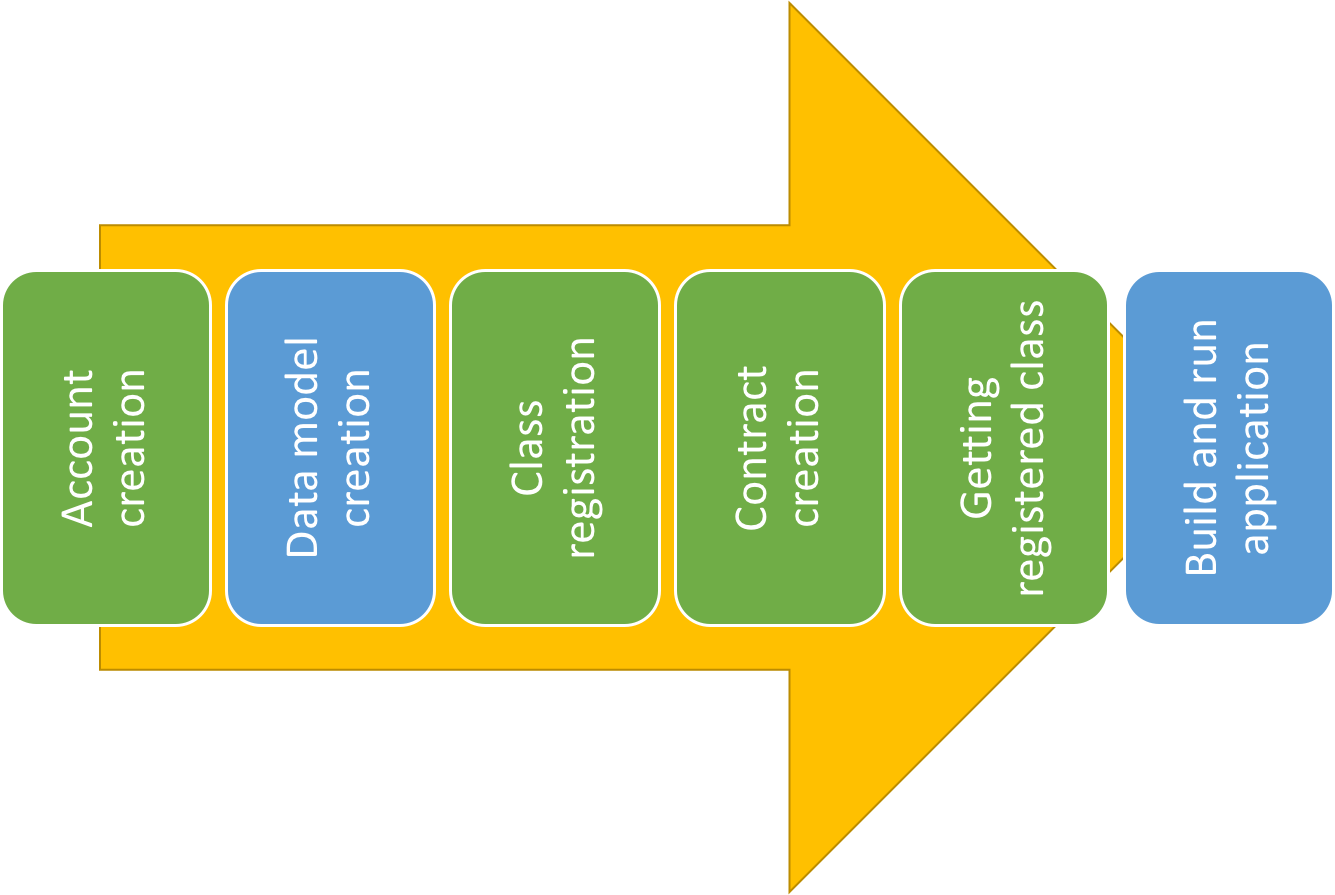
\includegraphics[scale=0.5]{FirstSteps/AppCycle.png}
\caption{Application life cycle}
\label{fig:AppCycle}
\end{figure}

\section{Account creation}\index{account}\index{account creation}

Everybody using dataClay needs to have its own account regardless of the role (model provider or application programmer). Currently accounts are identified by a string and are protected by a password. Accounts are the abstraction used to grant/deny privileges to create/use/access models and/or data.

Although dataClay foresees two different roles with respect to data, they can all be assumed by the same person and this is that case in the HelloPeople example: a single person (you) creates the model, creates application, and inserts the data.

Details on how accounts are created are presented in Chapter~\ref{sec:dClayTool}.

\section{Namespaces and class models}\index{class registration}
\label{sec:ClassRegistration}

The model provider is in charge of implementing the Java/Python class models. The involved classes are normally designed and implemented ignoring that they will be eventually used to store persistent objects in dataClay. Once the classes have been created and tested, the model provider needs to register them into dataClay to enable objects of these classes to be stored persistently.

Registering classes is important for three reasons: i) enables dataClay to automatically offer an optimal serialization of the objects instantiating any of these classes, ii) enables dataClay to execute class methods over the objects inside the backends without having to move data to the application, and iii) enables the sharing of classes among application developers in an easy and effective way.

Registering a class model only implies uploading its corresponding class files (e.g. .class files or .py files) into dataClay and defining into which namespace they should be added.

A {\bf namespace}\index{namespace} is a dataClay abstraction to group a set of classes together. Namespaces have two objectives: i) grouping related classes to ease the task of sharing them with other users and ii) avoiding class name clashing (for instance two users willing to register class models with names in common for a subset of their classes). That is, a namespace is a similar abstraction as a package in Java or module in Python.

Registering a class model can be easily performed by using the available tools described in Chapter~\ref{sec:dClayTool} and has to be performed before any application tries to store objects of this class model into dataClay.

% \section{Contract creation}\index{contract}\index{contract creation}
% 
% In order to be able to use data (actual objects) and models (classes), the application developer needs to have access to both the model and the data. In dataClay this access is allowed via model and data contracts.

% \subsection{Model contract}\index{model contract}\index{contract, model}
% 
% Model contracts allow application developers to use a given class or set of classes. These contracts can be of one of the following two types:
% 
% \begin{itemize}
% 	\item {\bf Public contract}:\index{public contract}\index{contract, public} is a contract that can be used by any dataClay user without explicit consent from the model developer. Thus any application programmer can use any class in a public contract. 
% 
% 	\item {\bf Private contract}:\index{private contract}\index{contract, private} is a contract that grants permission to use a set of classes to a specific user. Only the beneficiary user will be able to use these classes by means of this contract. A private contract may include many classes, a class may also be included in many contracts, and beneficiaries can have as many private contracts as needed to develop their applications.
% \end{itemize}
% 
% Contract creation can be easily performed by using the available tools described in Chapter~\ref{sec:dClayTool}. Once a model contract is created, dataClay will make sure that the user receiving the contract, or any user in case of a public contract, will have access to the classes included in the contract. An application can use as many models contracts as needed, and they can be a mix between public and private ones.

\section{Datasets and data contracts}\index{data contract}\index{contract, data}

In the same way we grouped classes into namespaces to ease the task of sharing them, dataClay also has the dataset abstraction. A {\bf dataset}\index{dataset} is a set of objects that will be shared with other users as a whole. Objects inside a dataset can be of any class and there is no restriction to the number of objects or their size inside a dataset. Datasets are identified by a string defined by the creator of the dataset.

Datasets can be public or private. Public datasets can be accessed by any user and they will suffice in most scenarios. On the contrary, to access a private dataset its owner has to explicitly grant permission to it. This permission granting is achieved by means of data contracts \index{data contract}. Contract creation can be easily performed by using the available tools described in Chapter~\ref{sec:dClayTool}. Once a data contract is created, dataClay will make sure that the user receiving the contract will have access to the objects included in the datasets of the contract. An application can access as many datasets as needed as will be shown in Chapter~\ref{sec:ClientConfigFiles} or Chapter~\ref{sec:FullDemo}.

Notice that in the current public version of dataClay, only public datasets are available.

\section{Using a registered class: getting its stubs}\index{stub}\index{class stub}

As we mentioned in Section~\ref{sec:ClassRegistration}, when we implement a class model we do not take into account anything about persistence, but when using it (as seen in the code in Section~\ref{sec:HelloPeople}), persistent objects have methods such as \texttt{makePersistent}\index{makePersistent} that have not been defined as part of the class. In order to be able to use such methods, and thus enable persistence of objects, the application needs to be linked with an automatically modified version of the classes. This modified version is what we refer as {\bf stub classes}\index{stub class} or simply {\bf stubs}\index{stub}. A stub is a class file containing the modified version of the original class in order to be compatible with dataClay. It is important to understand that, besides the newly added methods, the rest of the class behaves just like the original one. 

The stubs of a class are obtained using the available tools described in Chapter~\ref{sec:dClayTool}.

\section{Build and run the application}

To run a dataClay application, we just need i) to make sure that it is using the stubs instead of the original class files and ii) to create two configuration files that specify our account, datasets, stubs path and connection info. Next section shows an example of these configuration files and Section~\ref{sec:ClientConfigFiles} describes further details.

\section{Easier than it looks}

Let's see how we can execute the examples in Sections~\ref{sec:JavaFirstApp} and~\ref{sec:PythonFirstApp}.

First, we define two configuration files. Section~\ref{sec:ClientConfigFiles} describes further details and where to place them.

The first one is named \textit{session.properties}\index{session.properties} and the initialization method (\texttt{DataClay.init()}\index{DataClay.init()} in Java or \texttt{api.init()} in Python) will automatically process it. This initialization process is detailed in Section~\ref{sec:JavaGlobalAPI} for Java and Section~\ref{sec:PythonGlobalAPI} for Python.

Here is an example:

\begin{tBox}
\begin{bash}
Account=Alice
Password=AlicePass
DataSets=HelloPeopleDS
DataSetForStore=HelloPeopleDS
StubsClasspath=./stubs
\end{bash}
\end{tBox}

A second file named \textit{client.properties}\index{client.properties} contains the basic information for the network connection with dataClay:

\begin{tBox}
\begin{bash}
HOST=127.0.0.1
PORT=11034
\end{bash}
\end{tBox}

Now you can start using a simple dataClay tool\index{dClayTool} intended for management operations\index{management operations}. In this way, our class models can be registered, datasets with specific access rights can be defined, and our application can interact transparently with dataClay when using downloaded stubs (more details about the tool are explained in Chapter~\ref{sec:dClayTool}).

\begin{minipage}{\linewidth}
\begin{tBox}
\begin{bash}
 # To begin with, create an account
 dClayTool.sh NewAccount Alice AlicePass
 
 # Create a dataset (with granted access) 
 # to register stored objects on it
 dClayTool.sh NewDataContract Alice AlicePass myDataset
 
 # Register the class model in a certain namespace
 # Assuming Person.class or person.py is in ./modelClassDirPath
 dClayTool.sh NewModel Alice AlicePass myNamespace ./modelClassDirPath \
  <java | python>
 
 # Download the corresponding stubs for your application
 dClayTool.sh GetStubs Alice AlicePass myNamespace stubsDirPath
\end{bash}
\end{tBox}
\end{minipage}



\part{Java: Programmer API}
  \chapterimage{Coffee.jpg} % Chapter heading image

\chapter{Java API}
\label{sec:JavaAPI}

This chapter presents the Java API that can be used by applications divided into the following sections. First, in Section~\ref{sec:JavaGlobalAPI} we present the API intended to initialize and finish applications, as well as, to gather information about the system. In Section~\ref{sec:JavaObjectStore} we show the API for Object Store operations (GET(CLONE)/PUT/UPDATE). Next, in Section~\ref{sec:JavaObjectExtendedMethods} we introduce extended methods to expand object store operations from an Object-oriented programming perspective. In Section~\ref{sec:JavaObjectAdvanced} we show advanced extensions that will only be needed by a subset of applications. Finally, we present extra concepts such as error handling in Section~\ref{sec:JavaErrorHandling}, replica management in Section~\ref{sec:JavaReplication} and further considerations in Section~\ref{sec:JavaConsiderations}.

Notice that current supported Java version is 1.8 (OpenJDK 8, reference implementation of Java SE 8).

\section{dataClay API}
\label{sec:JavaGlobalAPI}

In this section, we present a set of calls that are not linked to any given object, but are general to the system.

In Java, they can be called through \textit{DataClay} main class by including the import:

\colorbox{basecolor!20}{\texttt{import es.bsc.dataclay.api.DataClay}}


% ------- finish ---------

\begin{dBox}
\texttt{public static void \CALL{finish}() throws DataClayException}
\LINE

{\it Description:}

\begin{itemize}
    \item Finishes a session with dataClay that has been previously created using init.
\end{itemize}

{\it Exceptions:}

\begin{itemize}
    \item If the session is not initialized or an error occurs while finishing the session, a DataClayException is thrown.
\end{itemize}
 
\end{dBox}


% ------- getBackends ---------

\begin{dBox}
\label{call:JavaGetBackends}
\texttt{public static Map<BackendID, Backend> \CALL{getBackends}() }
\LINE

{\it Description:}

\begin{itemize}
    \item Retrieves the available backends in the system.
\end{itemize}
 
{\it Returns:}

\begin{itemize}
    \item A map with the available backends in the system indexed by their backend IDs.
\end{itemize}

{\it Exceptions:}

\begin{itemize}
    \item If the session is not initialized, a DataClayException is thrown.
\end{itemize}

\end{dBox}


% ------- init ---------

\begin{dBox}
\texttt{public static void \CALL{init}() throws DataClayException}
\LINE

{\it Description:}

\begin{itemize}
    \item Creates and initializes a new session with dataClay.
\end{itemize}

{\it Environment:}

\begin{itemize}
    \item \texttt{\bfseries session.properties:} The configuration file can be optionally specified. Location of this file and its contents are detailed in Section~\ref{sec:ClientConfigFiles}.
\end{itemize}

{\it Exceptions:}

\begin{itemize}
    \item If any error occurs while initializing the session, a DataClayException is thrown.
\end{itemize}
 
\end{dBox}

\begin{tBox}
\textcolor{basecolor} {\bf Example: Using dataClay api - distributed people}
\begin{java}
import es.bsc.dataclay.api.DataClay;
import model.Person;

// Open session with init()
DataClay.init();

List<Person> people = new ArrayList<>();
people.add(new Person("Alice", 32));
people.add(new Person("Bob", 41));
people.add(new Person("Charlie", 35));

// Retrieve backend information with getBackends()
Map<BackendID, Backend> backends = DataClay.getBackends();

BackendID[] backendArray = backends.keySet().toArray();
int numBackends = backends.size();
int i = 0;
for (Person p : people) {
  p.dcPut(backendArray[i % numBackends]);
  i++;
}

// Close session with finish()
DataClay.finish();
\end{java}
\end{tBox}


\section{Object store methods}\index{Object Store}
\label{sec:JavaObjectStore}

Object store methods are those related to common \textit{GET(CLONE)/PUT/UPDATE} operations as introduced in Sections~\ref{sec:ExecutionModel} and \ref{sec:MyFirstApplication}.

Given that these three operations are very common in class model definition (e.g. get/put operations in collections), we prepend the ``dc'' prefix to prevent an unexpected behavior due to potential overriden operations. Notice that \textit{get} is named as \textit{dcClone} to match OO terminology.

This section focuses on a set of static methods that can be called directly from \textit{DataClayObject} class.



\subsection{Class methods}
\label{sec:JavaClassMethodsObjectStore}

The following methods can be called from any downloaded stub as static methods. In this way, the user is allowed to access persistent objects by using their aliases (see Section~\ref{sec:JavaObjectStoreStubMethods} to see how objects are persisted with an alias assigned). Aliases prevent objects to be removed by the Garbage Collector, thus an operation to remove the alias of an object is also provided. More details on how the garbage collector works can be found in Section~\ref{sec:GarbageCollection}. 

Notice that the examples provided assume the initialization and finalization of user's session with methods described in previous section Section~\ref{sec:JavaGlobalAPI}.

% ------- dcCloneByAlias ---------

\begin{dBox}
\texttt{public static <T> \CALL{dcCloneByAlias} (String alias [, boolean recursive]) \newline throws DataClayException}
\LINE

{\it Description:}

\begin{itemize}
    \item Retrieves a copy of current object from dataClay. Fields referencing to other objects are kept as remote references to objects stored in dataClay, unless the recursive parameter is set to \textit{True}.
\end{itemize}

{\it Parameters:}
\begin{itemize}
    \item \texttt{\bfseries alias:} alias of the object to be retrieved.
    \item \texttt{\bfseries recursive:} When this is set to True, the default behavior is altered so not only current object but all of its references are also retrieved locally.
\end{itemize}

{\it Returns:}

\begin{itemize}
    \item A new object instance initialized with the field values of the object with the alias specified.
\end{itemize}

{\it Exceptions:}

\begin{itemize}
    \item If no object with specified alias exists, a DataClayException is raised.
\end{itemize}

\end{dBox}

\begin{tBox}
\textcolor{basecolor} {\bf Example: Using dcCloneByAlias method}
\begin{java}
Person newPerson = new Person("Alice", 32);
newPerson.dcPut("student1");
Person retrieved = Person.dcCloneByAlias("student1");
assertTrue(retrieved.getName().equals(newPerson.getName())
\end{java}
\end{tBox}


% ------- dcUpdateByAlias ---------

\begin{dBox}
\texttt{public static void \CALL{dcUpdateByAlias} (String alias, \newline DataClayObject fromObject) throws DataClayException}
\LINE

{\it Description:}

\begin{itemize}
    \item Updates the object identified by specified alias with contents of \textit{fromObject}.
\end{itemize}

{\it Parameters:}
\begin{itemize}
    \item \texttt{\bfseries alias:} alias of the object to be retrieved.
    \item \texttt{\bfseries fromObject:} the base object which contents will be used to update target object with alias specified.
\end{itemize}

{\it Exceptions:}

\begin{itemize}
    \item If no object with specified alias exists, a DataClayException is raised.
    \item If object identified with given alias has different fields than \textit{fromObject}, a DataClayException is raised.
\end{itemize}

\end{dBox}

\begin{tBox}
\textcolor{basecolor} {\bf Example: Using dcUpdateByAlias method}
\begin{java}
Person newP = new Person("Alice", 32);
newP.dcPut("student1");
Person newValues = new Person("Alice Smith", 35);
Person.dcUpdateByAlias("student1", newValues);
Person clonedP = Person.cloneByAlias("student1");
assertTrue(clonedP.getName().equals(newValues.getName()));
\end{java}
\end{tBox}


\subsection{Object methods}
\label{sec:JavaObjectStoreStubMethods}

This section expands Section~\ref{sec:JavaClassMethodsObjectStore} with methods that can be called directly from object stub instances. That is, stub classes are adapted to extend a common dataClay class called DataClayObject, which provides the following methods.


% ------- dcClone ---------

\begin{dBox}
\texttt{public <T> \CALL{dcClone} (([boolean recursive]) throws DataClayException}
\LINE

{\it Description:}

\begin{itemize}
    \item Retrieves a copy of current object from dataClay. Fields referencing to other objects are kept as remote references to objects stored in dataClay.
\end{itemize}

{\it Parameters:}
\begin{itemize}
    \item \texttt{\bfseries recursive:} When this is set to True, the default behavior is altered so not only current object but all of its references are also retrieved locally.
\end{itemize}

{\it Returns:}

\begin{itemize}
    \item A new object instance initialized with the field values of current object. Non-primitive fields or sub-objects are also copied by creating new objects.
\end{itemize}

{\it Exceptions:}

\begin{itemize}
    \item If current object is not persistent, a DataClayException is raised.
\end{itemize}

\end{dBox}

\begin{tBox}
\textcolor{basecolor} {\bf Example: Using dcClone method}
\begin{java}
Person p = new Person("Alice", 32);
p.dcPut("student1");
Person copy = p.dcClone()
assertTrue(copy.getAge() == p.getAge())
\end{java}
\end{tBox}


% ------- dcPut ---------

\begin{dBox}
\texttt{public void \CALL{dcPut} () throws DataClayException}\index{alias}

\texttt{public void \CALL{dcPut} (String alias [, BackendID backendID]) \newline throws DataClayException}\index{alias}

\texttt{public void \CALL{dcPut} (String alias [, boolean recursive]) \newline throws DataClayException}\index{alias}

\texttt{public void \CALL{dcPut} (String alias, BackendID backendID
\newline [, boolean recursive]) throws DataClayException}\index{alias}
\LINE

{\it Description:}

\begin{itemize}
    \item Stores an aliased object in the system and assigns an OID to it. Notice this method allows specifying a certain backend. In this regard, the \colorbox{basecolor!15}{\texttt{\bfseries DataClay.LOCAL}} field can be set as a constant for a specific backendID (as detailed in Section~\ref{sec:ClientConfigFiles}). To use this field from your application, you have to add the proper import: \colorbox{basecolor!15}{\texttt{import es.bsc.dataClay.api.DataClay}}.
\end{itemize}

{\it Parameters:}

\begin{itemize}
    \item \texttt{\bfseries alias:} a string that will identify the object in addition to its OID. Aliases are unique in the system.
    \item \texttt{\bfseries backendID:} identifies the backend where the object will be stored. If this parameter is missing, then a random backend is selected to store the object. When \texttt{DataClay.LOCAL} is used, the object is created in the backend specified as local in the client configuration file.
    \item \texttt{\bfseries recursive:} when this flag is True, all objects referenced by the current one will also be made persistent (in case they were not already persistent) in a recursive manner. When this parameter is not set, the default behavior is to perform a recursive makePersistent.
\end{itemize}

{\it Exceptions:}

\begin{itemize}
    \item If there is a stored object with the same alias, a DataClayException is raised.
    \item If a backend is specified and it is not valid, a DataClayException is raised. Use getBackends (\ref{call:JavaGetBackends}) to obtain valid backends.
\end{itemize}

\end{dBox}

\begin{tBox}
\textcolor{basecolor} {\bf Example: Using dcPut method}
\begin{java}
Person p = new Person("Alice", 32);
p.dcPut("student1", DataClay.LOCAL);
assertTrue(p.getLocation().equals(DataClay.LOCAL));
\end{java}
\end{tBox}


% ------- dcUpdate ---------

\begin{dBox}
\texttt{public void \CALL{dcUpdate} (DataClayObject fromObject) throws DataClayException}
\LINE

{\it Description:}

\begin{itemize}
    \item Updates current object with contents of \textit{fromObject}.
\end{itemize}

{\it Parameters:}
\begin{itemize}
    \item \texttt{\bfseries fromObject:} the base object which contents will be used to update target object with alias specified.
\end{itemize}

{\it Exceptions:}

\begin{itemize}
    \item If object to be updated is not persistent, a DataClayException is raised.
    \item If the object has different fields than \textit{fromObject}, a DataClayException is raised.
\end{itemize}

\end{dBox}

\begin{tBox}
\textcolor{basecolor} {\bf Example: Using dcUpdate method}
\begin{java}
Person p = new Person("Alice", 32);
p.dcPut("student1");
Person newValues = new Person("Alice Smith", 35);
p.dcUpdate(newValues);
assertTrue(p.getName().equals(newValues.getName()));
\end{java}
\end{tBox}



\section{Object oriented methods}
\label{sec:JavaObjectExtendedMethods}

Besides object-store operations, dataClay also offers a set of methods to enable applications work in a more Object-oriented fashion. 

In Object-oriented programming objects are connected by using navigable associations (object references). In dataClay, applications might have objects containing fields associated with other persistent objects through remote object references. Therefore, a set of extended methods are provided to expand object store methods presented in previous section \ref{sec:JavaObjectStore}.


\subsection{Class methods}
\label{sec:JavaClassMethods}

% ------- deleteAlias ---------

\begin{dBox}
\texttt{public static void \CALL{deleteAlias} (String alias) \newline throws DataClayException}\index{alias}
\LINE

{\it Description:}

\begin{itemize}
    \item Removes the alias linked to an object. If this object is not referenced starting from a root object and no active session is accessing it, the garbage collector will remove it from the system.
\end{itemize}


{\it Parameters:}

\begin{itemize}
    \item \texttt{\bfseries alias:} alias to be removed.
\end{itemize}

{\it Exceptions:}

\begin{itemize}
    \item If no object with specified alias exists, a DataClayException is raised.
\end{itemize}

\end{dBox}

\begin{tBox}
\textcolor{basecolor} {\bf Example: Using deleteAlias}
\begin{java}
Person newPerson = new Person("Alice", 32);
newPerson.makePersistent("student1");
...
Person.deleteAlias("student1");
\end{java}
\end{tBox}


% ------- getByAlias ---------

\begin{dBox}
\texttt{public static void <T> \CALL{getByAlias} (String alias) \newline throws DataClayException}\index{alias}
\LINE

{\it Description:}

\begin{itemize}
    \item Retrieves an object reference of current stub class corresponding to the persistent object with alias provided.
\end{itemize}

{\it Parameters:}

\begin{itemize}
    \item \texttt{\bfseries alias:} alias of the object.
\end{itemize}

{\it Exceptions:}

\begin{itemize}
    \item If no object with specified alias exists, a DataClayException is raised.
\end{itemize}

\end{dBox}

\begin{tBox}
\textcolor{basecolor} {\bf Example: Using getByAlias }
\begin{java}
Person newPerson = new Person("Alice", 32);
newPerson.makePersistent("student1");
Person refPerson = Person.getByAlias("student1");
assertTrue(newPerson.getName().equals(refPerson.getName())
\end{java}
\end{tBox}



\subsection{Object methods}

In Object-oriented programming, aliases are not required if we can refer to an object by following a navigable association from another object. Therefore, the following method is similar to \textit{dcPut} but offering the possibility to register an object without an alias.

% ------- makePersistent ---------

\begin{dBox}
\label{sec:JavaObjecMakePersistent}
\texttt{public void \CALL{makePersistent} () throws DataClayException}\index{alias}

\texttt{public void \CALL{makePersistent} (BackendID backendID) \newline throws DataClayException}\index{alias}

\texttt{public void \CALL{makePersistent} (String alias, [BackendID backendID]) \newline throws DataClayException}\index{alias}

\texttt{public void \CALL{makePersistent} (String alias, [boolean recursive]) \newline throws DataClayException}\index{alias}

\texttt{public void \CALL{makePersistent} (BackendID backendID, [boolean recursive]) \newline  throws DataClayException}\index{alias}

\texttt{public void \CALL{makePersistent} (String alias, BackendID backendID, 
\newline [boolean recursive]) throws DataClayException}\index{alias}
\LINE

{\it Description:}

\begin{itemize}
    \item Stores an object in dataClay and assigns an OID to it.
\end{itemize}

{\it Parameters:}

\begin{itemize}
    \item \texttt{\bfseries alias:} a string that will identify the object in addition to its OID. Aliases are unique in the system. If no alias is set, this object will not have an alias, will only be accessible though other object references.
    \item \texttt{\bfseries backendID:} identifies the backend where the object will be stored. If this parameter is missing, then a random backend is selected to store the object. When \texttt{DataClay.LOCAL} is used, the object is created in the backend specified as local in the client configuration file.
    \item \texttt{\bfseries recursive:} when this flag is True, all objects referenced by the current one will also be made persistent (in case they were not already persistent) in a recursive manner. When this parameter is not set, the default behavior is to perform a recursive makePersistent.
\end{itemize}

{\it Exceptions:}

\begin{itemize}
    \item If an alias is specified and there is a stored object with the same alias, a DataClayException is raised.
    \item If a backend is specified and it is not valid, a DataClayException is raised. Use getBackends (\ref{call:JavaGetBackends}) to obtain valid backends.
\end{itemize}

\end{dBox}

\begin{tBox}
\textcolor{basecolor} {\bf Example: Using makePersistent method}
\begin{java}
Person p = new Person("Alice", 32);
p.makePersistent("student1", DataClay.LOCAL);
assertTrue(p.getLocation().equals(DataClay.LOCAL));
\end{java}
\end{tBox}



\section{Advanced methods}
\label{sec:JavaObjectAdvanced}

In this section we present advanced methods that are also inherited from DataClayObject class. These methods are not intended to be used by standard programmers, but by runtime and library developers or expert programmers.


% ------- getAllLocations ---------

\begin{dBox}
\texttt{public Set<BackendID> \CALL{getAllLocations}() throws DataClayException}
\LINE

{\it Description:}

\begin{itemize}
    \item Retrieves all locations where the object is persisted/replicated.
\end{itemize}

{\it Returns:}

\begin{itemize}
    \item A set of backend IDs in which this object or its replicas are stored.
\end{itemize}

{\it Exceptions:}

\begin{itemize}
    \item If the object is not persistent, a DataClayException is raised.
\end{itemize}

\end{dBox}

\begin{tBox}
\textcolor{basecolor} {\bf Example: Using getAllLocations}
\begin{java}
Person p1 = Person.getByAlias("personalias");
Set<BackendID> locations = p1.getAllLocations();
if (!locations.contains(DataClay.LOCAL)) {
 p1.newReplica(DataClay.LOCAL);
}
\end{java}
\end{tBox}


% ------- getLocation ---------

\begin{dBox}
\texttt{public BackendID \CALL{getLocation}() throws DataClayException}
\LINE

{\it Description:}

\begin{itemize}
    \item Retrieves a location of the object. % The returned location is one randomly picked from all locations where the object or a replica are stored.
\end{itemize}
 
{\it Returns:}

\begin{itemize}
    \item Backend ID in which this object is stored. If the object is not persistent (i.e. it has never been persisted) this function will fail.
\end{itemize}

{\it Exceptions:}

\begin{itemize}
    \item If the object is not persistent, a DataClayException is raised.
\end{itemize}

\end{dBox}

\begin{tBox}
\textcolor{basecolor} {\bf Example: Using getLocation}
\begin{java}
Person p1 = Person.getByAlias("student1");
p1.makePersistent(DataClay.LOCAL);
assertTrue(p1.getLocation().equals(DataClay.LOCAL));
\end{java}
\end{tBox}


% ------- newReplica ---------

\begin{dBox}

\texttt{public BackendID \CALL{newReplica}() throws DataClayException}

\texttt{public BackendID \CALL{newReplica}(boolean recursive) throws DataClayException}

\texttt{public BackendID \CALL{newReplica}(BackendID backendID \newline [,boolean recursive]) throws DataClayException}
\LINE

{\it Description:}

\begin{itemize}
    \item Creates a replica of the current object.
    
    It is important to notice that dataClay does not take care of replica synchronization. Details on how such synchronization can be achieved are described in Section~\ref{sec:JavaReplication}.
    \newline
    \newline
    Notice that the replication of an object includes the replication of its subobjects (references) as the default behavior (i.e. recursive is True by default). Therefore, some objects (including current object) might be already present in the destination backend. These objects will be ignored from replication, since a backend cannot have two replicas of the same object. But it is ensured that, after a correct execution of this method, a full copy of the current object (and all its subobjects if recursive) is present in the returned backend (same as backendID if user specifies it).

\end{itemize}

{\it Parameters:}

\begin{itemize}
    \item \texttt{\bfseries backendID:} ID of the backend in which to create the replica. If null, a random backend is chosen. When \texttt{DataClay.LOCAL} is used, the object is replicated in the backend specified as local in the client configuration file.
    \item \texttt{\bfseries recursive:} when this flag is True, all objects referenced by the current one will also be replicated (except those that are already present in the destination backend). When this parameter is not set, the default behavior is to perform a recursive replica.
\end{itemize}

{\it Returns:}

\begin{itemize}
    \item The ID of the backend in which the replica was created. 
\end{itemize}

{\it Exceptions:}

\begin{itemize}
    \item If the object is not persistent, a DataClayException is raised.
    \item If a backend is specified and it is not valid, a DataClayException is raised. Use getBackends (\ref{call:JavaGetBackends}) to obtain valid backends.
\end{itemize}

\end{dBox}

\begin{tBox}
\textcolor{basecolor} {\bf Example: Using newReplica}
\begin{java}
Person p1 = Person.getByAlias("student1");
// replicating object and referenced objects
// from one of its locations to LOCAL
p1.newReplica(p1.getLocation(), DataClay.LOCAL);
\end{java}
\end{tBox}


% ------- runRemote --------

\begin{dBox}
\texttt{public Object \CALL{runRemote}(BackendID location, \newline String opID, Object[] params) throws DataClayException}
\LINE

{\it Description:}

\begin{itemize}
    \item Executes a specific method on a particular backend. Notice that currently this method is intended for synchronization purposes, as can be seen in
  section \ref{sec:JavaReplication}. Check that section for a proper example.
\end{itemize}

{\it Parameters:}

\begin{itemize}
    \item \texttt{\bfseries location:} Backend where the method must be executed. When \texttt{DataClay.LOCAL} is used, the execution request is sent to the backend specified as local in the client configuration file.
    \item \texttt{\bfseries opID:} ID of the method to be executed.
    \item \texttt{\bfseries params:} The regular parameters of the method.
\end{itemize}
 
{\it Returns:}

\begin{itemize}
    \item The expected result from the execution of the specified method.
\end{itemize}

{\it Exceptions:}

\begin{itemize}
    \item If this object is not persistent, a DataClayException is raised.
    \item If location specified is not valid, a DataClayException is raised. Use getBackends (\ref{call:JavaGetBackends}) to obtain valid backends.
\end{itemize}

\end{dBox}


% ------- moveObject ---------

%\begin{dBox}
%\texttt{public void \CALL{moveObject}(BackendID sBackendID, BackendID dBackendID \newline [,boolean recursive]) throws DataClayException}
%\LINE
%
%{\it Description:}
%
%\begin{itemize}
%  \item Moves the object (or replica) from a backend identified by sBackendID to another backend identified by dBackendID.
%\end{itemize}
%
%{\it Parameters:}
%
%\begin{itemize}
%  \item \texttt{\bfseries sBackendID:} ID of the source location in which the object is stored.
%  \item \texttt{\bfseries dBackendID:} ID of the destination location in which the object should be moved. 
%  \item \texttt{\bfseries recursive:} when this flag is True, all objects referenced by the current one will also be moved. When this parameter is not set, the default behavior is to perform a recursive move.
%\end{itemize}
%
%{\it Exceptions:}
%
%\begin{itemize}
%  \item If the object is not persistent, the object is not located int he source location, or any of the location IDs do not represent a valid location, a DataClayException is raised.
%\end{itemize}
% 
%\end{dBox}
%
%\begin{tBox}
%\textcolor{basecolor} {\bf Example: Using moveObject}
%\begin{lstlisting}
%Person p1 = Person.getByAlias("student1");
%// moving object, but not referenced objects, from one of its locations to LOCAL
%p1.moveObject(p1.getLocation(), DataClay.LOCAL, false);
%\end{lstlisting}
%\end{tBox}

\section {Error management}\index{error management}
\label{sec:JavaErrorHandling}

Besides \textit{DataClayException} raised from \textit{DataClayObject} methods or dataClay API methods as exposed along this chapter, exceptions raised from methods of your class models while running on a dataClay backend are also forwarded to end-user applications.

However, notice that current version of dataClay does not allow you to register your own exception classes (i.e. as part of your data model), so methods enclosed in your data model can only throw language built-in exceptions.

\section {Memory Management and Garbage Collection}\index{garbage collection}\index{memory management}

In section \ref{sec:GarbageCollection} we introduced the routines that aim to optimize memory and disk usage in the backends.

In Java, users cannot deallocate objects manually so in dataClay we do not provide a direct operation to do so. However, since we add an extra layer for persistence we have to ensure that the Java Garbage Collector (GC) does not remove loaded objects before they are synchronized with the underlying storage. To this end, a dataClay thread periodically checks if the memory usage reaches a certain threshold and, when this is the case, objects are firstly flushed to persistent storage in a way that Java GC can collect them.

On the other hand, a Global Garbage Collector keeps track of global reference counters in a per object basis. Considering the conditions that an object has to meet in order to be removed, as stated in section \ref{sec:GarbageCollection}, its associated reference counter not only counts which objects are pointing to it, but also how many aliases it has or the applications and running methods that are using it.

In some cases, certain objects used in long-running applications, such as services, are only needed during a limited period of time, and it may be convenient to free the space they are taking. The following method can be used to notify the Global Garbage Collector that an object is no longer needed by the application or service and, thus, it can be garbage-collected: 

\begin{dBox}
\texttt{public final void \CALL{sessionDetach}()}
\LINE

{\it Description:}

\begin{itemize}
  \item Dissociates current object from the current session. 
\end{itemize}

{\it Parameters:}

\end{dBox}


\section{Replica management}\index{replica management}
\label{sec:JavaReplication}

Given that each object or piece of data may potentially need a different consistency model, dataClay will not synchronize objects. On the other hand, it will offer mechanisms for the model developer to include it as part of the model in an easy way, and how to be able to import the consistency model form another class already defined.

The first way to guarantee the consistency level required by a replicated object is to add the needed code in all setters/getter of the class. Although this is a feasible option is quite impractical if we need to add this code to all classes we want to build. Fir this reason, dataClay also offers a mechanism to add arbitrary code (from a static class) to be executed before or after a given method. This mechanism, explained in detail in this section, will enable programmers to build their consistency model once (or use a predefined one) and use it in any of their classes without modifying the class itself.

In this section, we present how to add consistency code into existing classes.

Let us assume that we have our class Person:

\begin{tBox}
\begin{java}
public class Person {
  String name;
  int age;
  public Person(String name, int age) {
    this.name = name;
    this.age = age;
  }
}
\end{java}
\end{tBox}

Once this class is registered and with the proper permissions and stubs, an application that uses it might look like this:

\begin{tBox}
\begin{java}
public class App {
  public static void main(String[] args) {
    DataClay.init();
    Person p = new Person("Alice", 42);
    
    p.makePersistent("student1");
    p.newReplica();
    
    p.setAge(43);
    System.out.println(p.getAge());
  }
}
\end{java}
\end{tBox}

With no consistency policies, the printed message would show an unpredictable age for Alice, since methods \textit{setAge} and \textit{getAge} are executed in a random backend among the locations of the object.

In order to overcome this problem, dataClay provides a mechanism to define synchronization policies at user-level. In particular, class developers are allowed to define three different annotations to customize the behavior of attribute updates:

\begin{tBox}
\begin{java}
    @Replication.InMaster
    @Replication.BeforeUpdate(method="...", clazz="...")
    @Replication.AfterUpdate(method="...", clazz="...")
\end{java}
\end{tBox}

The \textit{InMaster} annotation forces the update operation to be handled from the master location. The default master location of an object is the backend where the object was originally stored.

On the other hand, \textit{BeforeUpdate} and \textit{AfterUpdate} define extra behavior to be executed before or after the update operation. The \textit{method} argument specifies an operation signature of a static class method. The \textit{clazz} argument refers to the class where such a static class method is implemented. In this way, the developer is allowed to define an action to be triggered before the update operation, and an action to be taken after the update operation.

Let us resume our previous example. Assuming that the \textit{name} attribute is never modified (e.g. private setter), we want, however, that every time the age is updated the change is propagated to all the replicas. Empowering Person class with the proper annotation, we can intervene updates of attribute \textit{age} to perform the update synchronization:

\begin{tBox}
\begin{java}
public class Person {
  String name;

  @Replication.InMaster
  @Replication.AfterUpdate(method="replicateToSlaves",
                                    clazz="model.SequentialConsistency")
  int age;
  public Person(String name, int age) {
    this.name = name;
    this.age = age;
  }
}
\end{java}
\end{tBox}

Following the example, and as part of the class model, the proposed \textit{SequentialConsistency} class can be implemented as follows:

\begin{tBox}
\begin{java}
package model;

import java.util.Set;

import api.BackendID;
import serialization.DataClayObject;

public class SequentialConsistency {
  public static void replicateToSlaves(DataClayObject o, String setter, Object[] args) {
    Set<BackendID> locations = o.getAllLocations();
    for (BackendID replicaLocation : locations) {
      if (!replicaLocation.equals(o.getMasterLocation())) {
         o.runRemote(replicaLocation, setter, args);
      }
    }
  }
}
\end{java}
\end{tBox}

In this example, the master replica leads a sequential consistency model by synchronizing the contents with secondary replicas. 

Some considerations merit the attention of model developers:

\begin{itemize}
    \item The master location of an object can be checked with the method \textit{getMasterLocation()}.
    \item The method name specified in the annotations is always implemented as a \textit{public static void} operation, which receives the context info about the original method that triggered the action. This context info consists of:
 \begin{itemize}
    \item A dataClay object reference. Object in which the original method is being executed. In our example, a reference to Person object.
    \item The method itself. An identifier that dataClay can manage. In our example, the \textit{setAge} method identifier.
    \item The arguments received by the method. In our example, the new age to be set.
 \end{itemize}
\end{itemize}

For convenience, the implementation of the \textit{SequentialConsistency} class in the example can be used by including the import:

\colorbox{basecolor!20}{\texttt{import es.bsc.dataclay.util.replication.Replication}}

\FEDERATION{
\section{Federation}\index{federation}
\label{sec:jFederation}

In some scenarios, such as edge-to-cloud environments, part of the data stored in a dataClay instance has to be shared with another dataClay instance running in a different device. An example can be found in the context of smart cities where, for instance, part of the data residing in a car is temporarily shared with the city the car is traversing. This partial, and possibly temporal, integration of data between independent dataClay instances is implemented by means of dataClay's federation mechanism.
More precisely, federation consists in replicating an object (either simple or complex, such as a collection of objects) in an independent dataClay instance so that the recipient dataClay can access the object without the need to contact the owner dataClay. This provides immediate access to the object, avoiding communications when the object is requested and overcoming the possible unavailability of the data source. 

An object can be federated with an unlimited number of other dataClay instances. Additionally, a dataClay instance that receives a federated object can federate it with other dataClay instances.

Federated objects can be synchronized in all dataClay instances sharing them, in such a way that only those parts of the data that change are transferred through the network in order to avoid unnecessary transfers. This is achieved analogously to the synchronization of replicas stored among different backends of a single dataClay, as explained below. 

To federate an object, both the source and the target dataClay must have the same data model registered. This is achieved by importing the model from the target dataClay, or from another dataClay instance holding the same model as the target dataClay. This process is done through the methods \textit{RegisterDataClay} and \textit{ImportModelsFromExternalDataClay} (as well as the usual \textit{GetStubs}) before the execution of the application (see Section \ref{sec:dClayTool}).

In this section we present how to manage federation of objects that instantiate Java classes. 

Assume we have our class Person:

\begin{tBox}
\begin{java}
public class Person {
  String name;
  int age;
  public Person(String name, int age) {
    this.name = name;
    this.age = age;
  }
}
\end{java}
\end{tBox}

An application that federates an object of this class with another dataClay might look like this:

\begin{tBox}
\begin{java}
import es.bsc.dataclay.api.DataClay;

public class App {
  public static void main(String[] args) {
    DataClay.init();
    otherDC = DataClay.registerDataClay(host, port)
    
    Person p = new Person("Alice", 42);
    p.makePersistent("person1");
    
    p.federate(otherDC); 
  }
}
\end{java}
\end{tBox}

The first step is to make both dataClay instances aware of each other by means of the \textit{registerDataClay} method, explained in section \ref{sec:JavaFederationAPI}. The dataClay instance id returned by this call is used as a parameter for the \textit{federate} call on the object to indicate the dataClay instance that will receive the federated object. As explained above, note that both dataClay instances must have the same data model registered. 
At this point, an application accessing the dataClay instance \textit{otherDC} can execute the following code:

\begin{tBox}
\begin{java}
public class App {
  public static void main(String[] args) {
    DataClay.init();
    
    Person p = Person.getByAlias("person1");
    
    System.out.println(p.name);
  }
}
\end{java}
\end{tBox}

The secondary dataClay has actually performed a replica of Person object aliased \textit{person1}. From now on, this 
replica can be used in the execution environment of any of the backends of the secondary dataClay, as any other object created in \textit{otherDC}.

A user-defined behaviour can optionally be attached to the class of the object to be federated, which will be executed upon reception of the object in the target dataClay instance. To do this, a method \textit{whenFederated} must be implemented in the corresponding class, for instance:

\begin{tBox}
\begin{java}
public class Person {
  String name;
  int age;
 
 public Person(String name, int age) {
    this.name = name;
    this.age = age;

 public whenFederated() {
    PersonList pl = PersonList.getByAlias("persons"); 
    pl.add(this);
  }
}
\end{java}
\end{tBox}

In this way, the application accessing the target dataClay instance can use the collection \textit{pl} to get all the available objects of class \textit{Person} at any time. Notice that \textit{pl} is not a federated object, but a collection residing in the target dataClay instance that includes objects federated from the source dataClay (as well as possibly other objects created in the target dataClay instance).

\begin{tBox}
\begin{java}
public class App {
  public static void main(String[] args) {
    ...
    
    PersonList pl = new PersonList();
    pl.makePersistent("persons");
    ...
    length = pl.size();
    ...
  }
}
\end{java}
\end{tBox}
 
Federated objects can be synchronized using the same mechanisms provided to synchronize replicas within a dataClay instance, as explained in \ref{sec:JavaReplication}. To implement customized synchronization mechanisms on federated objects, the methods to be used are \textit{getFederationTargets}, which returns the identifiers of the dataClay instances where the object is federated, and \textit{getFederationSource}, which returns the source dataClay instance of a federated object in the current dataClay. Also, the method \textit{setInBackend} is provided to execute a setter method on the replica of the object that is stored in the specified dataClay instance. The description of these methods can be found in section \ref{sec:JavaFederationObject}.

For convenience, to synchronize federated objects following a sequential consistency policy, the method \textit{synchronizeFederated} in the same \textit{SequentialConsistency} class can be used.

Both the source and the target dataClay instance can stop sharing an object by calling the \textit{unfederate} method on the federated object. Then, the replica in the target dataClay will be eventually removed by the garbage collector unless it has an alias or it is referenced by another object. In any case, it will cease to be synchronized with the original object. 

Analogously to federation, the method \textit{whenUnfederated} can be implemented in the corresponding class to execute a customized behaviour in the target dataClay instance when an object is unfederated (for instance, removing the object from the \textit{PersonList} in the example above, so that the object can be garbage-collected.

\FEDERATION{
\section{Federation mechanism}
\label{sec:JavaObjectFederation}

More details about federation are presented in Section~\ref{sec:jFederation}.

% ------- federate ---------
\begin{dBox}
\texttt{public void \CALL{federate}(DataClayInstanceID dcID [,boolean recursive])}
\LINE

{\it Description:}

\begin{itemize}
  \item Federates current object with another dataClay instance. 
\end{itemize}

{\it Parameters:}

\begin{itemize}
  \item \texttt{\bfseries dcID:} ID of the external dataClay. It must be previously registered.
  \item \texttt{\bfseries recursive:} when this flag is TRUE, all objects (recursively) referenced by the current one will also be federated (except those that are already present in the destination dataClay). This parameter is optional, default value is TRUE.
\end{itemize}

\end{dBox}

\begin{tBox}
\textcolor{basecolor} {\bf Example: Using federate}
\begin{java}
DataClayID otherDC = DataClay.getDataClayID(host, port);
Person p1 = Person.getByAlias("person1");
// federating object and subobjects to otherDC (previously registered)
p1.federate(otherDC);
\end{java}
\end{tBox}

% ------- getFederationSource ------

\begin{dBox}
\texttt{public DataClayInstanceID \CALL{getFederationSource}()}
\LINE

{\it Description:}

\begin{itemize}
 \item Retrieves the ID of the dataClay instance where the object is federated from. 
\end{itemize}

{\it Returns:}

\begin{itemize}
 \item A DataClayInstanceID which is the source of this federated object.  
 It is null if the object is not federated.
\end{itemize}

\end{dBox}

% ------- getFederationTargets ------

\begin{dBox}
\texttt{public Set<DataClayInstanceID> \CALL{getFederationTargets}()}
\LINE

{\it Description:}

\begin{itemize}
 \item Retrieves the IDs of all the dataClay instances where the object is federated to. 
\end{itemize}

{\it Returns:}

\begin{itemize}
 \item A set of DataClayInstanceID objects in which this object is federated. 
 It is empty if the object is not federated.
\end{itemize}

\end{dBox}

\begin{tBox}
\textcolor{basecolor} {\bf Example: Using getFederationTargets}
\begin{java}
Person p1 = Person.getByAlias("personalias");
// using getFederationTargets to check if p1 is federated
Set<DataClayInstanceID> federation = p1.getFederationTargets();
return (!federation.size() == 0)
\end{java}
\end{tBox}

% ------- synchronizeFederated --------

\begin{dBox}
\texttt{public void \CALL{synchronizeFederated}(DataClayInstanceID dcID, \newline ImplementationID implID, Object[] params)} 
\LINE

{\it Description:}

\begin{itemize}
  \item Executes an implementation on a particular dataClay where the object is federated, for synchronization purposes.
\end{itemize}

{\it Parameters:}

\begin{itemize}
  \item \texttt{\bfseries dcID:} dataClay instance where the method must be executed.
  \item \texttt{\bfseries pimlID:} ID of the implementation to be executed.
  \item \texttt{\bfseries params:} The parameters of the method.
\end{itemize}
 
\end{dBox}

% ------- unfederate ---------
\begin{dBox}

\texttt{public void \CALL{unfederate}([DataClayInstanceID dcID] [,boolean recursive])}
\LINE

{\it Description:}

\begin{itemize}
  \item Unfederates current object (and referenced objects) with the indicated dataClay instance. If no dataClayID is specified, the object is unfederated from all the instances where it lives.
\end{itemize}

{\it Parameters:}

\begin{itemize}
  \item \texttt{\bfseries dcID:} ID of the external dataClay. It must be previously registered.
  \item \texttt{\bfseries recursive:} when this flag is TRUE, all objects (recursively) referenced by the current one will also be unfederated. This parameter is optional, default value is TRUE.
\end{itemize}

\end{dBox}


}
}

\section{Further considerations}
\label{sec:JavaConsiderations}

This section exposes some particularities that are coupled to current dataClay requirements or limitations.

% Current version of dataClay has some unsupported features for Java class models. Most significant ones are listed below.
% 
% \begin{enumerate}
%  \item Non-final static attributes or class attributes. Only final static attributes are supported.
%  \item User-defined interfaces. Only language predefined interfaces can be implemented.
%  \item Non-distributed \texttt{synchronized}. You can code a \texttt{synchronized} method or statement, but they will be only effective in a per backend basis. That is, \texttt{synchronize} on a method or object will not behave as a distributed lock.
%  \item Assertions. Due to its exceptional behavior, currently we are not providing \texttt{assert} support since it will require special flags to execute JVM on dataClay backends.
%  \item Third-party libraries. You can assume that classes from JDK 1.8 (i.e. \textit{java.util.*}) are available for your data models, but current version of dataClay does not support the registration of external jar files.
%  \item Handover of lambda functions. Lambdas can only be used in the context of a single execution environment. That is, lambdas cannot be passed in remote execution requests.
%  \item User-defined exceptions. You can throw Java exceptions from methods of your registered class models, but you cannot define your own Exceptions as part of your class model.
%  \item Handover of non-serializable Java classes. They can be used within a method (e.g. Iterators), but cannot be passed as argument or returned as result.
% \end{enumerate}


\subsection{Importing registered classes}
\label{sec:JavaImports}

In order to use certain classes from registered data models you will have to specify the imports for the corresponding stubs. To this end, you have to ensure that Java \textit{classpath} includes the path of your stubs directory when running your applications.

\subsection{Non-registered classes}
Non-registered mutable types (such as Java built-in collections) are opaque to dataClay. Thus, when a registered class has one of such objects (as a field) and this mutable object is modified from outside its containing class, the changes in the mutable object may not be reflected.

For example, given a Class A with a field b of type B, and B has a field list of type \texttt{ArrayList}. After executing the instruction \texttt{this.b.list.add(x)} from a method in A, the list may not contain the new element x. To solve this, the class model should define a method in class B containing the instruction \texttt{b.list.add(x)} and call it from class A.

\subsection{Third party libraries}

Sometimes using third-party libraries from registered data models is not trivial, thus if you experience such problems, please contact us by email: \texttt{\href{mailto:support-dataclay@bsc.es}{support-dataclay@bsc.es}}

\FILTERING{
\section{Collection filtering}\index{filtering}
\label{sec:JavaFiltering}

\TODO{Check it makes sense}
\TODO{Python filtering}
\TODO{Check Grammar is correct}
\TODO{Maybe we could decide a unique method for filtering, currently we have two or more for non-AST queries}

A user class implementing the \textit{Iterable} interface can benefit from filtering methods provided by DataClay objects (i.e. from the corresponding stubs).

The method to filter an iterable object, i.e. a collection, only requires a query in String format compliant with the following grammar:

\begin{lstlisting}
 Filter  ::= ( AndExpr )or( Filter )*
 
 AndExpr ::= ( Comp )and( AndExpr )*
 
 Comp    ::= Attribute Op Value
         | Value Op Attribute
         | Filter
 
 Op      ::= '<' | '<=' | '=' | '>=' | '>' | '!=' | ':=' | '^='
 
 Attribute ::= ? attribute name possibly nested ?
 
 Value ::=IntValue | DateValue | StringValue | BoolValue

 IntValue ::= /[0-9]+/ | -/[0-9]+/
 DateValue ::= ? in Java standard String format ?
 StringValue ::= "..." | '...'
 BoolValue ::= 'true' | 'false'
\end{lstlisting}

The following example illustrates a basic class model representing an iterable collection of Person objects (following HelloPeople example in section \ref{sec:HelloPeople}) to filter them afterwards.

\begin{tBox}
\texttt{\bfseries\textcolor{basecolor}{HelloPeople.java}}
\begin{lstlisting}[language=Java]
package model;
import model.Person;
import java.util.Iterator;
import java.util.List;
import java.util.ArrayList;

public class PersonList implements Iterable<Person> {
    public List<Person> people;

    public People() {
      people = new ArrayList<>();
    }
    
    @Override
    public Iterator<Person> iterator() {
      return people.iterator();
    }
}

\end{lstlisting}
\end{tBox}

This basic class could be filled with Person objects and once registered and obtained the corresponding stub, you will be enabled to execute the following method.

\begin{dBox}
\texttt{public List<Object> \CALL{filterStream}(final String conditions)}
\LINE

{\it Description:}

\begin{itemize}
  \item If 'this' object is iterable (i.e. its class implements Iterable interface), the query is applied by iterating through the object and checking the provided conditions. Objects found matching these conditions are returned in a List.
\end{itemize}

{\it Parameters:}

\begin{itemize}
  \item \texttt{\bfseries conditions:} The query conditions matching the previously presented grammar.
\end{itemize}
 
{\it Returns:}

\begin{itemize}
  \item The list of objects that match the conditions specified within the query.
\end{itemize}

{\it Exceptions:}

\begin{itemize}
  \item If this object is not Iterable.
\end{itemize}

\end{dBox}
}

%  \chapterimage{Coffee.jpg} % Chapter heading image

\chapter{Management API}
\label{sec:JavaManagementAPI}

\DISCUSS{Jon: I do not know what Toni wants here, is not dClayTool?}

%  \chapterimage{Coffee.jpg} % Chapter heading image

\chapter{Project specific API}

\TODO{brief intro to this chapter}

\section{COMPSs specific API}

In this section we present extensions to the dataClay API needed to improve the integration with the COMPSs programming model~\cite{Tejedor_2008}\cite{Tejedor_2015}, also developed at BSC.


\TODO{Add calls such as new version, consolidate, ...}

% ------- getID ---------

\begin{dBox}
\texttt{public java.lang.String \CALL{getID}() throws StorageException}
\LINE

{\it Description:}

\begin{itemize}
	\item Retrieves the object ID of the current object in string format. This specific format is needed to be used in other API calls such as ...
\end{itemize}

\TODO{Add the list of call that can use this format}
 
{\it Returns:}

\begin{itemize}
	\item Returns an OID (in string format) that identified the caller object. If the object is not persistent (i.e. it has never been persisted) this function will fail.
\end{itemize}

\TODO{What does it mean it fails? How does the programmer know, a return value, an exception, ...}
\end{dBox}

\begin{tBox}
\textcolor{basecolor} {\bf Example: Using getID}
\begin{verbatim}

Code

\end{verbatim}
\end{tBox}

\TODO{getBackendsByHostname}

\TODO{Fill the getID example}

\TODO{getByID}

\TODO{newReplica}

\TODO{ids2String}

\TODO{string2IDs}


%
%  \chapterimage{Coffee.jpg} % Chapter heading image

\chapter{Undocumented calls}

Under construction


\part{Python: Programmer API}
  \chapterimage{Python.jpg} % Chapter heading image

\chapter{Python API}
\label{sec:PythonAPI}

This chapter presents the Python API that can be used by applications divided into the following sections. First, in Section~\ref{sec:PythonGlobalAPI} we present the API intended to initialize and finish applications, as well as, to gather information about the system. In Section~\ref{sec:PythonObjectStore} we show the API for Object Store operations (GET(CLONE)/PUT/UPDATE). Next, in Section~\ref{sec:PythonObjectExtendedMethods} we introduce extended methods to expand object store operations from an Object-oriented programming perspective. In Section~\ref{sec:PythonObjectAdvanced} we show advanced extensions that will only be needed by a subset of applications. Finally, we present extra concepts such as error handling in Section~\ref{sec:PythonErrorHandling}, replica management in Section~\ref{sec:PythonReplication} and further considerations in Section~\ref{sec:PythonConsiderations}.

Notice that current supported Python versions are 2 and 3, but all the backends in the system, as well as the clients, should use the same Python major version (Section~\ref{sec:SystemInstall} describes further details about this).

\section{Global API}
\label{sec:PythonGlobalAPI}

In this section, we present a set of calls that are not linked to any given object, but are general to the system.

In Python, they can be called through \textit{dataclay.api} with the proper import:

\colorbox{basecolor!15}{\texttt{from dataclay.api import finish, init, get\_backends}}


% ------- finish ---------

\begin{dBox}
\texttt{def \CALL{finish}():}
\LINE

{\it Description:}

\begin{itemize}
    \item Finishes a session with dataClay that has been previously created using init.
\end{itemize}

{\it Exceptions:}

\begin{itemize}
    \item If the session is not initialized or an error occurs while finishing the session, a DataClayException is thrown.
\end{itemize}
 
\end{dBox}


% ------- getBackends ---------

\begin{dBox}
\label{call:PythonGetBackends}
\texttt{def \CALL{get\_backends}(): }
\LINE

{\it Description:}

\begin{itemize}
    \item Retrieves the available backends in the system.
\end{itemize}

{\it Returns:}

\begin{itemize}
    \item A map with the available backends in the system indexed by their IDs.
\end{itemize}

\begin{itemize}
    \item If the session is not initialized, a DataClayException is thrown.
\end{itemize}

\end{dBox}


% ------- init ---------

\begin{dBox}
\texttt{def \CALL{init}(config\_file='./cfgfiles/session.properties'):}
\LINE

{\it Description:}

\begin{itemize}
    \item Creates and initializes a new session with dataClay.
\end{itemize}

{\it Environment:}

\begin{itemize}
    \item \texttt{\bfseries session.properties:} The configuration file can be optionally specified. Location of this file and its contents are detailed in Section~\ref{sec:ClientConfigFiles}.
\end{itemize}

{\it Exceptions:}

\begin{itemize}
    \item If any error occurs while initializing the session, a DataClayException is thrown.
\end{itemize}
 
\end{dBox}

\begin{tBox}
\textcolor{basecolor} {\bf Example: Using global api - distributed people}
\begin{python}
from itertools import cycle
from dataclay.api import finish, init, get_backends

# Open session with init()
init()

from model import Person

student1 = Person(name="Alice", age=32)
person2 = Person(name="Bob", age=41)
person2 = Person(name="Charlie", age=35)
people = [p1, p2, p3]

# Retrieve backend information with get_backends()
backends = get_backends().keys()

# Round robin of persons in backends
for person, backend in zip(people, cycle(backends)):
    person.dc_put(backend_id=backend)

# Close session with finish()
finish()
\end{python}
\end{tBox}


\section{Object store methods}\index{Object Store}
\label{sec:PythonObjectStore}

Object store methods are those related to common \textit{GET(CLONE)/PUT/UPDATE} operations as introduced in Sections~\ref{sec:ExecutionModel} and \ref{sec:MyFirstApplication}.

Given that these three operations are very common in class model definition (e.g. get/put operations in collections), we prepend the ``dc'' prefix to prevent an unexpected behavior due to potential overriden operations. Notice that \textit{get} is named as \textit{dc\_clone} to match OO terminology.

This section focuses on a set of static methods that can be called directly from \textit{DataClayObject} class.



\subsection{Class methods}
\label{sec:PythonClassMethodsObjectStore}

The following methods can be called from any downloaded stub as class methods. In this way, the user is allowed to access persistent objects by using their aliases (see Section~\ref{sec:PythonObjectStoreStubMethods} to see how objects are persisted with an alias assigned). Aliases prevent objects to be removed by the Garbage Collector, thus an operation to remove the alias of an object is also provided. More details on how the garbage collector works can be found in Section~\ref{sec:GarbageCollection}. 

Notice that the examples provided assume the initialization and finalization of user's session with methods described in previous section Section~\ref{sec:PythonGlobalAPI}.

% ------- dc_clone_by_alias ---------

\begin{dBox}
\texttt{def \CALL{dc\_clone\_by\_alias} (cls, alias, recursive=False):}
\LINE

{\it Description:}

\begin{itemize}
    \item Retrieves a copy of current object from dataClay. Fields referencing to other objects are kept as remote references to objects stored in dataClay, unless the recursive parameter is set to \textit{True}.
\end{itemize}

{\it Parameters:}
\begin{itemize}
    \item \texttt{\bfseries alias:} alias of the object to be retrieved.
    \item \texttt{\bfseries recursive:} When this is set to True, the default behavior is altered so not only current object but all of its references are also retrieved locally.
\end{itemize}

{\it Returns:}

\begin{itemize}
    \item A new object instance initialized with the field values of the object with the alias specified.
\end{itemize}

{\it Exceptions:}

\begin{itemize}
    \item If no object with specified alias exists, a DataClayException is raised.
\end{itemize}

\end{dBox}

\begin{tBox}
\textcolor{basecolor} {\bf Example: Using dc\_clone\_by\_alias method}
\begin{java}
new_person = Person(name="Alice", age=32)
new_person.dc_put("student1")
retrieved = Person.dc_clone_by_alias("student1")
assert retrieved.get_name() == new_person.get_name()
\end{java}
\end{tBox}


% ------- dc_update_by_alias ---------

\begin{dBox}
\texttt{def \CALL{dc\_update\_by\_alias} (cls, alias, from\_object):}
\LINE

{\it Description:}

\begin{itemize}
    \item Updates the object identified by specified alias with contents of \textit{from\_object}.
\end{itemize}

{\it Parameters:}
\begin{itemize}
    \item \texttt{\bfseries alias:} alias of the object to be retrieved.
    \item \texttt{\bfseries from\_object:} the base object which contents will be used to update target object with alias specified.
\end{itemize}

{\it Exceptions:}

\begin{itemize}
    \item If no object with specified alias exists, a DataClayException is raised.
    \item If object identified with given alias has different fields than \textit{from\_object}, a DataClayException is raised.
\end{itemize}

\end{dBox}

\begin{tBox}
\textcolor{basecolor} {\bf Example: Using dc\_update\_by\_alias method}
\begin{java}
new_person = new Person(name="Alice", age=32)
new_person.dc_put("student1")
new_values = Person(name="Alice Smith", age=35)
Person.dc_update_by_alias("student1", new_values)
cloned_person = Person.dc_clone_by_alias("student1")
assert cloned_person.get_name() == new_values.get_name()
\end{java}
\end{tBox}



\subsection{Object methods}
\label{sec:PythonObjectStoreStubMethods}

This section expands Section~\ref{sec:PythonClassMethodsObjectStore} with methods that can be called directly from object instances. That is, stub classes are adapted to extend a common dataClay class called DataClayObject, which provides the following methods.


% ------- dc_clone ---------

\begin{dBox}
\texttt{def \CALL{dc\_clone} (recursive=False)}
\LINE

{\it Description:}

\begin{itemize}
    \item Retrieves a copy of current object from dataClay. Fields referencing to other objects are kept as remote references to objects stored in dataClay.
\end{itemize}

{\it Parameters:}
\begin{itemize}
    \item \texttt{\bfseries recursive:} When this is set to True, the default behavior is altered so not only current object but all of its references are also retrieved locally.
\end{itemize}

{\it Returns:}

\begin{itemize}
    \item A new object instance initialized with the field values of current object. Non-primitive fields or sub-objects are also copied by creating new objects.
\end{itemize}

{\it Exceptions:}

\begin{itemize}
    \item If current object is not persistent, a DataClayException is raised.
\end{itemize}

\end{dBox}

\begin{tBox}
\textcolor{basecolor} {\bf Example: Using dc\_clone method}
\begin{java}
new_person = Person(name="Alice", age=32)
new_person.dc_put("student1")
copy = new_person.dc_clone()
assert copy.get_age() == new_person.get_age()
\end{java}
\end{tBox}


% ------- dc_put ---------

\begin{dBox}
\texttt{def \CALL{dc\_put} (self, alias, backend\_id=None, recursive=True):}\index{alias}
\LINE

{\it Description:}

\begin{itemize}
    \item Stores an aliased object in the system and assigns an OID to it. Notice that next method allows specifying a certain backend. In this regard, the \colorbox{basecolor!15}{\texttt{\bfseries api.LOCAL}} field can be set as a constant for a specific backendID (as detailed in Section~\ref{sec:ClientConfigFiles}). To use this field from your application, you have to add the proper import: \colorbox{basecolor!15}{\texttt{from dataclay import api}}.
\end{itemize}

{\it Parameters:}

\begin{itemize}
    \item \texttt{\bfseries alias:} a string that will identify the object in addition to its OID. Aliases are unique in the system.
    \item \texttt{\bfseries backendID:} identifies the backend where the object will be stored. If this parameter is missing, then a random backend is selected to store the object. When \texttt{api.LOCAL} is used, the object is created in the backend specified as local in the client configuration file.
    \item \texttt{\bfseries recursive:} when this flag is True, all objects referenced by the current one will also be made persistent (in case they were not already persistent) in a recursive manner. When this parameter is not set, the default behavior is to perform a recursive makePersistent.
\end{itemize}

{\it Exceptions:}

\begin{itemize}
    \item If there is a stored object with the same alias, a DataClayException is raised.
    \item If a backend is specified and it is not valid, a DataClayException is raised. Use get\_backends (\ref{call:PythonGetBackends}) to obtain valid backends.
\end{itemize}

\end{dBox}

\begin{tBox}
\textcolor{basecolor} {\bf Example: Using dc\_put method}
\begin{java}
new_person = Person(name="Alice", age=32)
new_person.dc_put("student1", api.LOCAL)
locations = list(p1.get_all_locations())
assert api.LOCAL in locations
\end{java}
\end{tBox}


% ------- dc_update ---------

\begin{dBox}
\texttt{def \CALL{dc\_update} (self, from\_object)}
\LINE

{\it Description:}

\begin{itemize}
    \item Updates current object with contents of \textit{from\_object}.
\end{itemize}

{\it Parameters:}
\begin{itemize}
    \item \texttt{\bfseries from\_object:} the base object which contents will be used to update target object with alias specified.
\end{itemize}

{\it Exceptions:}

\begin{itemize}
    \item If object to be updated is not persistent, a DataClayException is raised.
    \item If the object has different fields than \textit{from\_object}, a DataClayException is raised.
\end{itemize}

\end{dBox}

\begin{tBox}
\textcolor{basecolor} {\bf Example: Using dc\_update method}
\begin{java}
new_person = Person(name="Alice", age=32)
new_person.dc_put("student1")
new_values = Person(name="Alice Smith", age=35)
new_person.dc_update(new_values)
assert new_person.get_name() == new_values.get_name()
\end{java}
\end{tBox}



\section{Object oriented methods}
\label{sec:PythonObjectExtendedMethods}

Besides object store operations, dataClay also offers a set of methods to enable applications work in a more Object-oriented fashion. 

In Object-oriented programming objects are connected by using navigable associations (object references). In dataClay, applications might have objects containing fields associated with other persistent objects through remote object references. Therefore, a set of extended methods are provided to expand object store methods presented in previous section \ref{sec:PythonObjectStore}.


\subsection{Class methods}
\label{sec:PythonClassMethods}

% ------- delete_alias ---------

\begin{dBox}
\texttt{def \CALL{delete\_alias}(cls, alias):}\index{alias}
\LINE

{\it Description:}

\begin{itemize}
    \item Removes the alias linked to an object. If this object is not referenced starting from a root object and no active session is accessing it, the garbage collector will remove it from the system.
\end{itemize}


{\it Parameters:}

\begin{itemize}
    \item \texttt{\bfseries alias:} alias to be removed.
\end{itemize}

{\it Exceptions:}

\begin{itemize}
    \item If no object with specified alias exists, a DataClayException is raised.
\end{itemize}

\end{dBox}

\begin{tBox}
\textcolor{basecolor} {\bf Example: Using delete\_alias}
\begin{python}
new_person = Person(name="Alice", age=32)
new_person.make_persistent("student1")
...
Person.delete_alias("student1")
\end{python}
\end{tBox}


% ------- get_by_alias ---------

\begin{dBox}
\texttt{def \CALL{get\_by\_alias}(cls, alias):}\index{alias}
\LINE

{\it Description:}

\begin{itemize}
    \item Retrieves an object reference of current stub class corresponding to the persistent object with alias provided.
\end{itemize}

{\it Parameters:}

\begin{itemize}
    \item \texttt{\bfseries alias:} alias of the object.
\end{itemize}

{\it Exceptions:}

\begin{itemize}
    \item If no object with specified alias exists, a DataClayException is raised.
\end{itemize}

\end{dBox}

\begin{tBox}
\textcolor{basecolor} {\bf Example: Using get\_by\_alias }
\begin{python}
new_person = Person(name="Alice", age=32)
new_person.make_persistent("student1")
ref_person = Person.get_by_alias("student1")
assert new_person.get_name() == ref_person.get_name()
\end{python}
\end{tBox}



\subsection{Object methods}

In Object-oriented programming, aliases are not required if we can refer to an object by following a navigable association from another object. Therefore, the following method is similar to \textit{dc\_put} but offering the possibility to register an object without an alias.

% ------- make_persistent ---------

\begin{dBox}
\label{sec:PythonObjectMakePersistent}
\texttt{def \CALL{make\_persistent}(self, alias=None, backend\_id=None, recursive=True):}\index{alias}
\LINE

{\it Description:}

\begin{itemize}
    \item Stores an object in dataClay and assigns an OID to it.
\end{itemize}

{\it Parameters:}

\begin{itemize}
    \item \texttt{\bfseries alias:} a string that will identify the object in addition to its OID. Aliases are unique in the system. If no alias is set, this object will not have an alias, will only be accessible though other object references.
    \item \texttt{\bfseries backend\_id:} identifies the backend where the object will be stored. If this parameter is missing, then a random backend is selected to store the object. When \texttt{api.LOCAL} is used, the object is created in the backend specified as local in the client configuration file.
    \item \texttt{\bfseries recursive:} when this flag is True, all objects referenced by the current one will also be made persistent (in case they were not already persistent) in a recursive manner. When this parameter is not set, the default behavior is to perform a recursive makePersistent.
\end{itemize}

{\it Exceptions:}

\begin{itemize}
    \item If an alias is specified and there is a stored object with the same alias, a DataClayException is raised.
    \item If a backend is specified and it is not valid, a DataClayException is raised. Use get\_backends (\ref{call:PythonGetBackends}) to obtain valid backends.
\end{itemize}

\end{dBox}

\begin{tBox}
\textcolor{basecolor} {\bf Example: Using make\_persistent}
\begin{python}
p1 = Person(name="Alice", age=32)
p1.make_persistent("student1", api.LOCAL)
assert p1.get_location() == api.LOCAL
\end{python}
\end{tBox}



\section{Advanced methods}
\label{sec:PythonObjectAdvanced}

In this section we present advanced methods that are also inherited from DataClayObject class. These methods are not intended to be used by standard programmers, but by runtime and library developers or expert programmers.


% ------- get_all_locations ---------

\begin{dBox}
\texttt{def \CALL{get\_all\_locations}(self):}
\LINE

{\it Description:}

\begin{itemize}
    \item Retrieves all locations where the object is persisted/replicated.
\end{itemize}

{\it Returns:}

\begin{itemize}
    \item A set of backend IDs in which this object or its replicas are stored.
\end{itemize}

{\it Exceptions:}

\begin{itemize}
    \item If the object is not persistent, a DataClayException is raised.
\end{itemize}

\end{dBox}

\begin{tBox}
\textcolor{basecolor} {\bf Example: Using get\_all\_locations}
\begin{python}
new_person = Person(name="Alice", age=32)
new_person.make_persistent("student1", api.LOCAL)
locations = list(p1.get_all_locations())
assert api.LOCAL in locations
\end{python}
\end{tBox}


% ------- getLocation ---------

\begin{dBox}
\texttt{def \CALL{get\_location}(self):}
\LINE

{\it Description:}

\begin{itemize}
    \item Retrieves a location of the object. % The returned location is one randomly picked from all locations where the object or a replica are stored.
\end{itemize}
 
{\it Returns:}

\begin{itemize}
    \item Backend ID in which this object is stored. If the object is not persistent (i.e. it has never been persisted) this function will fail.
\end{itemize}

{\it Exceptions:}

\begin{itemize}
    \item If the object is not persistent, a DataClayException is raised.
\end{itemize}

\end{dBox}

\begin{tBox}
\textcolor{basecolor} {\bf Example: Using get\_location}
\begin{python}
new_person = Person(name="Alice", age=32)
new_person.make_persistent("student1", api.LOCAL)
assert new_person.get_location() == api.LOCAL
\end{python}
\end{tBox}


% ------- newReplica ---------

\begin{dBox}
\texttt{def \CALL{new\_replica}(self, backend\_id=None, recursive=True):}
\LINE

{\it Description:}

\begin{itemize}
    \item Creates a replica of the current object.
    
    It is important to notice that dataClay does not take care of replica synchronization. Details on how such synchronization can be achieved are described in Section~\ref{sec:PythonReplication}.
    \newline
    \newline
    Notice that the replication of an object includes the replication of its subobjects (references) as the default behavior (i.e. recursive is True by default). Therefore, some objects (including current object) might be already present in the destination backend. These objects will be ignored from replication, since a backend cannot have two replicas of the same object. But it is ensured that, after a correct execution of this method, a full copy of the current object (and all its subobjects if recursive) is present in the returned backend (same as backend\_ID if user specifies it).

\end{itemize}

{\it Parameters:}

\begin{itemize}
    \item \texttt{\bfseries backend\_id:} ID of the backend in which to create the replica. If null, a random backend is chosen. When \texttt{api.LOCAL} is used, the object is replicated in the backend specified as local in the client configuration file.
    \item \texttt{\bfseries recursive:} when this flag is True, all objects referenced by the current one will also be replicated (except those that are already present in the destination backend). When this parameter is not set, the default behavior is to perform a recursive replica.
\end{itemize}

{\it Returns:}

\begin{itemize}
    \item The ID of the backend in which the replica was created. 
\end{itemize}

{\it Exceptions:}

\begin{itemize}
    \item If the object is not persistent, a DataClayException is raised.
    \item If a backend is specified and it is not valid, a DataClayException is raised. Use get\_backends (\ref{call:PythonGetBackends}) to obtain valid backends.
\end{itemize}

\end{dBox}

\begin{tBox}
\textcolor{basecolor} {\bf Example: Using new\_replica}
\begin{python}
p1 = Person.get_by_alias("student1")
# replicating object and referenced objects
# from one of its locations to LOCAL
p1.new_replica(api.LOCAL)
\end{python}
\end{tBox}


% ------- runRemote --------

\begin{dBox}
\texttt{def \CALL{run\_remote}(backend\_id, operation\_name, params)}
\LINE

{\it Description:}

\begin{itemize}
    \item Executes a specific method on a particular backend. Notice that currently this method is intended for synchronization purposes, as can be seen in
  section \ref{sec:PythonReplication}. Check that section for a proper example.
\end{itemize}

{\it Parameters:}

\begin{itemize}
    \item \texttt{\bfseries backend\_id,:} Backend where the method must be executed. When \texttt{api.LOCAL} is used, the execution request is sent to the backend specified as local in the client configuration file.
    \item \texttt{\bfseries operation\_name:} Method to be executed.
    \item \texttt{\bfseries params:} The regular parameters of the method.
\end{itemize}
 
{\it Returns:}

\begin{itemize}
    \item The expected result from the execution of the specified method.
\end{itemize}

{\it Exceptions:}

\begin{itemize}
    \item If this object is not persistent, a DataClayException is raised.
    \item If location specified is not valid, a DataClayException is raised. Use get\_backends (\ref{call:PythonGetBackends}) to obtain valid backends.
\end{itemize}

\end{dBox}

\FEDERATION{
In the following we present the API provided by dataClay to manage the federation of objects between dataClay instances. It comprises a set of methods that are part of the dataClay API to manage the connection between different dataClay instances, as well as object methods to manage the federation of objects. Recall that methods from the dataClay API can be called through \textit{dataclay.api} with the proper import, for instance:

\colorbox{basecolor!20}{\texttt{from dataclay.api import finish, init, register\_dataclay}}

\subsection{dataClay API methods}
\label{sec:PythonFederationAPI}

% ------- getDataClayID ---------

\begin{dBox}
\texttt{def \CALL{get\_dataclay\_id}([host, port]):}
\LINE

{\it Description:}

\begin{itemize}
    \item Retrieves the ID of the dataClay instance accessible in \textit{host}, \textit{port}, or of the current dataClay instance if there are no parameters.
\end{itemize}

{\it Parameters:}

\begin{itemize}
  \item \texttt{\bfseries host:} host where the dataClay instance is located.
  \item \texttt{\bfseries port:} port where the dataClay instance is listening.
\end{itemize}

{\it Returns:}

\begin{itemize}
 \item The ID of the current dataClay instance, or of the dataClay instance located in \textit{host}, \textit{port}.
\end{itemize}

\end{dBox}

% ------- registerDataClay ---------

\begin{dBox}
\texttt{def \CALL{register\_dataclay}(host, port):}
\LINE

{\it Description:}

\begin{itemize}
    \item Makes the current dataClay instance aware of another dataClay instance accessible in \textit{host} and \textit{port}, and returns its ID.
\end{itemize}

{\it Parameters:}

\begin{itemize}
  \item \texttt{\bfseries host:} host where the dataClay instance to be registered is located.
  \item \texttt{\bfseries port:} port where the dataClay instance to be registered is listening.
\end{itemize}

{\it Returns:}

\begin{itemize}
 \item The ID of the dataClay instance located in \textit{host}, \textit{port}.
\end{itemize}

\end{dBox}

% ------- federate ---------
\begin{dBox}
\texttt{def \CALL{federate}(self, dc\_id, recursive=True):}
\LINE

{\it Description:}

\begin{itemize}
  \item Federates current object with another dataClay instance, replicating it in any of its backends. 
\end{itemize}

{\it Parameters:}

\begin{itemize}
  \item \texttt{\bfseries dc\_id:} ID of the external dataClay. It must be previously registered.
  \item \texttt{\bfseries recursive:} when this flag is TRUE, all objects (recursively) referenced by the current one will also be federated (except those that are already present in the destination dataClay). 
\end{itemize}
\end{dBox}


\begin{tBox}
\textcolor{basecolor} {\bf Example: Using federate}
\begin{python}
  other_dc = get_dataclay_id(host, port);
  p1 = Person.get_by_alias("person1");
  # federating object and subobjects to other_dc (previously registered)
  p1.federate(other_dc);
\end{python}
\end{tBox}

% ------- federateToBackend ---------
\begin{dBox}
\texttt{def \CALL{federate\_to\_backend}(self, backend\_id, recursive=True):}
\LINE

{\it Description:}

\begin{itemize}
  \item Federates current object with another dataClay instance, replicating it in the indicated backend.
\end{itemize}

{\it Parameters:}

\begin{itemize}
  \item \texttt{\bfseries backend\_id:} ID of a backend in an external dataClay instance, which must be previously registered.
  \item \texttt{\bfseries recursive:} when this flag is TRUE, all objects (recursively) referenced by the current one will also be federated (except those that are already present in the destination dataClay). 
\end{itemize}
\end{dBox}

% ------- getFederationSource ------

\begin{dBox}
\texttt{def \CALL{get\_federation\_source}(self):}
\LINE

{\it Description:}

\begin{itemize}
 \item Retrieves the ID of the dataClay instance where the object is federated from. 
\end{itemize}

{\it Returns:}

\begin{itemize}
 \item The id of the dataClay instance that is the source of this federated object.  
 It is null if the object is not federated.
\end{itemize}

\end{dBox}

% ------- getFederationTargets ---------

\begin{dBox}
\texttt{def \CALL{get\_federation\_targets}(self):}
\LINE

{\it Description:}

\begin{itemize}
 \item Retrieves the IDs of all the dataClay instances where the object is federated. 
\end{itemize}

{\it Returns:}

\begin{itemize}
 \item A set of DataClayInstanceID objects in which this object is federated. 
 It can be empty if it is not federated.
\end{itemize}

\end{dBox}

\begin{tBox}
\textcolor{basecolor} {\bf Example: Using get\_federation\_targets}
\begin{python}
from dataclay import api
newPerson = Person.get_by_alias('Alias')
dataclays = list(p1.get_federation_of_object())
assert api.LOCAL in dataclays
\end{python}
\end{tBox}

% ------- setInDataClayInstance ---------

\begin{dBox}
\texttt{def \CALL{set\_in\_dataclay\_instance}(self, dc\_id, operation\_name, params):}
\LINE

{\it Description:}

\begin{itemize}
  \item Executes a setter on a particular dataClay where the object is federated.
\end{itemize}

{\it Parameters:}

\begin{itemize}
  \item \texttt{\bfseries dc\_id:} dataClay instance where the method must be executed.
  \item \texttt{\bfseries operation\_name:} ID of the setter to be executed.
  \item \texttt{\bfseries params:} The parameters of the method.
\end{itemize}
 
\end{dBox}

% ------- unfederate ---------
\begin{dBox}

\texttt{def \CALL{unfederate}(self, [dc\_id], recursive=True):}
\LINE

{\it Description:}

\begin{itemize}
  \item Unfederates current object (and referenced objects) with the indicated dataClay instance. If no \textit{dc\_id} is specified, the object is unfederated from all the instances where it lives.
\end{itemize}

{\it Parameters:}

\begin{itemize}
  \item \texttt{\bfseries dc\_id:} ID of the external dataClay. It must be previously registered.
  \item \texttt{\bfseries recursive:} when this flag is TRUE, all objects (recursively) referenced by the current one will also be unfederated.
\end{itemize}

\end{dBox}







}



% ------- moveObject ---------

%\begin{dBox}
%\texttt{def \CALL{move\_object}(self, source\_backend\_id, dest\_backend\_id, recursive):}
%\LINE
%
%\TODO{NOT IMPLEMENTED}
%
%{\it Description:}
%
%\begin{itemize}
%    \item Moves the object (or replica) from a backend identified by source\_backend\_id to another backend identified by  dest\_backend\_id.
%\end{itemize}
%
%{\it Parameters:}
%
%\begin{itemize}
%    \item \texttt{\bfseries source\_backend\_id:} ID of the source backend in which the object is stored.
%    \item \texttt{\bfseries dest\_backend\_id:} ID of the destination backend in which the object should be moved. 
%    \item \texttt{\bfseries recursive:} when this flag is True, all objects referenced by the current one will also be moved. When this parameter is not set, the default behavior is to perform a recursive move.
%\end{itemize}
%
%{\it Exceptions:}
%
%\begin{itemize}
%    \item If the object is not persistent, the object is not located int he source location, or any of the location IDs do not represent a valid location, a DataClayException is raised.
%\end{itemize}
% 
%\end{dBox}
%
%\begin{tBox}
%\textcolor{basecolor} {\bf Example: Using move\_object}
%\begin{python}
%p1 = get_by_alias(Person, "student1")
%# moving object, but not referenced objects, from one of its locations to LOCAL
%p1.move_object(p1.get_location(), api.LOCAL, false)
%assert api.LOCAL in p1.get_all_locations()
%\end{python}
%\end{tBox}

\section {Error management}\index{error management}
\label{sec:PythonErrorHandling}

Besides \textit{DataClayException} raised from \textit{DataClayObject} methods or dataClay API methods as exposed along this chapter, exceptions raised from methods of your class models while running on a dataClay backend are also forwarded to end-user applications.

However, notice that current version of dataClay does not allow you to register your own exception classes (i.e. as part of your data model), so methods enclosed in your data model can only throw language built-in exceptions.

\section {Memory Management and Garbage Collection}\index{garbage collection}\index{memory management}

In section \ref{sec:GarbageCollection} we introduced the routines that aim to optimize memory and disk usage in the backends.

In Python, users cannot deallocate objects manually so dataClay does not provide a direct operation to do that. However, since we add an extra layer for persistence we have to ensure that Python does not remove objects before they are synchronized with the underlying storage. To this end, a dataClay thread periodically checks if the memory usage reaches a certain threshold and, when this is the case, objects are firstly flushed to persistent storage in a way that the Python GC can collect them.

On the other hand, a Global Garbage Collector keeps track of global reference counters in a per object basis. Considering the conditions that an object has to meet in order to be removed, as stated in section \ref{sec:GarbageCollection}, its associated reference counter not only counts which objects are pointing to it, but also how many aliases it has or the applications and running methods that are using it.

\section{Replica management}\index{replica management}
\label{sec:PythonReplication}

Given that each object or piece of data may potentially need a different consistency model, dataClay will not synchronize objects. On the other hand, it will offer mechanisms for the model developer to include it as part of the model in an easy way, and how to be able to import the consistency model form another class already defined.

The first way to guarantee the consistency level required by a replicated object is to add the needed code in all setters/getter of the class. Although this is a feasible option is quite impractical if we need to add this code to all classes we want to build. Fir this reason, dataClay also offers a mechanism to add arbitrary code ( fom a static class) to be executed before or after a given method. This mechanism, explained in detail in this section, will enable programmers to build their consistency model once (or use a predefined one) and use it in any of their classes without modifying the class itself.

In this section, we present how to add consistency code into existing classes.

Let us assume that we have our class Person:

\begin{tBox}
\begin{python}
class Person(DataClayObject):
    @dclayMethod(name="str", age="int")
    def __init__(self, name, age):
        self.name = name
        self.age = age
\end{python}
\end{tBox}

Once this class is registered and with the proper permissions and stubs, an application that uses it might look like this:

\begin{tBox}
\begin{python}
# Initialize dataClay
from dataclay.api import init, finish, get_backends
init()

from model.classes import *

if __name__ == "__main__":
    p = Person("foo", 100)
    backends = get_backends().keys()
    
    p.make_persistent(backend_id=backends[0])
    p.new_replica(backend_id=backends[1])    
    
    p.age = 1000
    print(p.age)    
    finish()
\end{python}
\end{tBox}

With no consistency policies, the printed message would show an unpredictable age for Alice, since getters and setters are executed in a random backend among the locations of the object.

In order to overcome this problem, dataClay provides a mechanism to define synchronization policies at user-level. In particular, class developers are allowed to define three different annotations to customize the behavior of attribute updates:

\begin{tBox}
\begin{python}
@dclayReplication(inMaster='boolean')
@dclayReplication(beforeUpdate='method')
@dclayReplication(afterUpdate='method')
@ClassField name type
\end{python}
\end{tBox}

The \textit{inMaster} annotation forces the update operation to be handled from the master location if set to true. The default master location of an object is the backend where the object was originally stored.

On the other hand, \textit{beforeUpdate} and \textit{afterUpdate} define extra behavior to be executed before or after the update operation. The \textit{method} argument specifies an operation signature of a method, which can belong to the same class or can be inherited from a mixin. In this way, the developer is allowed to define an action to be triggered before the update operation, and an action to be taken after the update operation.

The \textit{ClassField} annotation allows the user to define which fields of the class have to apply the defined behavior.

Let us resume our previous example. Assuming that the \textit{name} attribute is never modified (e.g. private setter), we want, however, that every time the \textit{age} is updated the change is propagated to all the replicas. Empowering Person class with the proper annotations, we can intervene updates of attribute \textit{age} to perform the update synchronization, which has been implemented in the class \textit{SequentialConsistencyMixin}, extended by \textit{Person}:

\begin{tBox}
\begin{python}
class Person(DataClayObject, SequentialConsistencyMixin):
    """ 
    @dclayReplication(afterUpdate='synchronize', inMaster='True')
    @ClassField age int
    """

    @dclayMethod(name="str", age="int")
    def __init__(self, name, age):
        self.name = name
        self.age = age

\end{python}
\end{tBox}

Following the example, and as part of the class model, the proposed \textit{SequentialConsistencyMixin} class can be implemented as follows:
\begin{tBox}
\begin{python}
class SequentialConsistencyMixin(object):

    @dclayMethod(attribute="str", value="anything")
    def synchronize(self, attribute, value):
        from dataclay.DataClayObjProperties import DCLAY_SETTER_PREFIX
        for exeenv_id in self.get_all_locations().keys():
            if exeenv_id != master_location:
                self.run_remote(exeenv_id, DCLAY_SETTER_PREFIX + attribute, value)

\end{python}
\end{tBox}

In this example, the master replica leads a sequential consistency model by synchronizing the contents with secondary replicas.

Some considerations merit the attention of model developers:

\begin{itemize}
    \item The master location can be checked through the field \textit{master\_location}.
    \item The method whose name is specified in the annotations is implemented in the model class or a superclass and receives the attribute name to be set and its new value.
\end{itemize}

For convenience,  the implementation of the \textit{SequentialConsistency} class in the example can be used by including the import:

\colorbox{basecolor!20}{\texttt{from dataClay.contrib.synchronization import SequentialConsistencyMixin}}

\section{Further considerations}
\label{sec:PythonConsiderations}

This section exposes some particularities that are coupled to current dataClay requirements or limitations.

\subsection{Type annotation}

Python uses dynamic typing and does not provide the concept of symbol table, therefore dataClay asks the model provider to explicitly specify the types for class registration.

To this end, fields, methods (argument and return types) and imports must be annotated, as you can notice in the examples of previous section \ref{sec:PythonReplication} about replica management. 

In particular, fields and imports are defined as part of the \textit{docstring} of the class, whereas methods are annotated using \textit{decorators}. 

In the case of imports, two tags are provided to define imports as shown in the examples below:

\begin{tBox}
 \begin{python}
  @dataClayImport numpy as np
  @dataClayImportFrom itertools import cycle
 \end{python}
\end{tBox}

In the case of fields and methods, they are annotated with tags \texttt{@ClassField} and \texttt{@dclayMethod} as shown, for instance, in People class from HelloPeople application:

\begin{tBox}
 \begin{python}
  class People(DataClayObject):
    """
    @ClassField people list<HelloPeople_ns.classes.Person>
    """
    @dclayMethod()
    def __init__(self):
        self.people = list()

    @dclayMethod(new_person="HelloPeople_ns.classes.Person")
    def add(self, new_person):
        self.people.append(new_person)

    @dclayMethod(return_="str")
    def __str__(self):
        result = ["People:"]

        for p in self.people:
            result.append(" - Name: %s, age: %d" % (p.name, p.age))

        return "\n".join(result)
 \end{python}
\end{tBox}

Notice that in case that a class requires types (classes) from your data models (registered or pending to register), you must provide a valid namespace as a prefix for your annotations. If the defined type belongs to a namespace that is pending to register (maybe because you are currently defining it) then you must ensure that the prefix used is the same as the namespace you will provide during the class model registration process.

In the example above, \textit{people} field is specified as a list of {\bf \texttt{HelloPeople\_ns.classes.Person}} objects being {\bf \texttt{HelloPeople\_ns}} the namespace to be used for the HelloPeople class model.

% Current version of dataClay has some unsupported features for Python class models. Most significant ones are listed below.
% 
% \TODO{Connected to TODO in error management section, it is said that DataClayException encapsulates any builtin exception to be passed, but Alex is not sure}
% 
% \begin{enumerate}
%  \item Class attributes and class methods. Attributes and methods can only be accessed at object level, you cannot execute a method or access an attribute from class context.
%  \item Generators and \texttt{yield} statement are not supported.
%  \item Handover of lambda functions. Lambdas can only be used in the context of a single execution environment. That is, lambdas cannot be passed in remote execution requests.
%  \item User-defined decorators. You cannot define your own decorators in Python methods.
%  \item Inheritance. Method overloading or multiple inheritance are not supported. You cannot call \texttt{super} method either.
%  \item Third-party libraries (except \texttt{numpy}). You can assume that classes from Python 2 are available for your data models, but current version of dataClay does not support the registration of external libraries. The only exception is for \texttt{numpy} which is registered by default in dataClay backends, enabling you to use it from your class models.
%  \item Arbitrary parameters \texttt{*args} and \texttt{**kwargs}.
%  \item Raising exceptions. You can handle exceptions within your methods with try except blocks, but they cannot be raised.
% \end{enumerate}

\subsection{Non-registered classes}
Non-registered mutable types (such as Python dictionaries or numpy arrays) are opaque to dataClay. Thus, when a registered class has one of such objects (as a field) and this mutable object is modified from outside its containing class, the changes in the mutable object may or may not be reflected.

For example, given a Class A with a field b of type B, and B has a list field. After executing the instruction \texttt{self.b.list.add(x)} from a method in A, the list may or may not contain the new element x. To solve this, the class model should define a method in class B containing the instruction \texttt{b.list.add(x)} and call it from class A.

\subsection{Third party libraries}

Sometimes using third-party libraries from registered data models is not trivial, thus if you experience such problems, please contact us by email: \texttt{\href{mailto:support-dataclay@bsc.es}{support-dataclay@bsc.es}}

\subsection{Execution environment}
\label{sec:PythonConsiderationsExecutionEnvironment}

Multithreading is supported both at the client side and at the server side. However, due to the CPython Global Interpreter Lock implementation details, only one thread can execute Python code at once (even though certain performance-oriented libraries might overcome this limitation). If you have Python-pure CPU-intensive parallel workloads which are being executed in methods of dataClay persisted objects, then you may experience serialization of executions (and thus, loss of performance).

In Section~\ref{sec:PythonParallelism} we explain how to face this problem, but if you still have some doubts or further requirements for your applications, please contact us (\texttt{\href{mailto:support-dataclay@bsc.es}{support-dataclay@bsc.es}}) and we will provide you the proper solutions.

\FEDERATION{
\section{Federation}\index{federation}
\label{sec:pFederation}

In some scenarios, such as edge-to-cloud environments, part of the data stored in a dataClay instance has to be shared with another dataClay instance running in a different device. An example can be found in the context of smart cities where, for instance, part of the data residing in a car is temporarily shared with the city the car is traversing. This partial, and possibly temporal, integration of data between independent dataClay instances is implemented by means of dataClay's federation mechanism.
More precisely, federation consists in replicating an object (either simple or complex, such as a collection of objects) in an independent dataClay instance so that the recipient dataClay can access the object without the need to contact the owner dataClay. This provides immediate access to the object, avoiding communications when the object is requested and overcoming the possible unavailability of the data source. 

An object can be federated with an unlimited number of other dataClay instances. Additionally, a dataClay instance that receives a federated object can federate it with other dataClay instances.

Federated objects can be synchronized in all dataClay instances sharing them, in such a way that only those parts of the data that change are transferred through the network in order to avoid unnecessary transfers. This is achieved analogously to the synchronization of replicas stored among different backends of a single dataClay, as explained below. 

To federate an object, both the source and the target dataClay must have the same data model registered. This is achieved by importing the model from the target dataClay, or from another dataClay instance holding the same model as the target dataClay. This process is done through the methods \textit{RegisterDataClay} and \textit{ImportModelsFromExternalDataClay} (as well as the usual \textit{GetStubs}) before the execution of the application (see Section \ref{sec:dClayTool}).

In this section, we present how to manage federation of objects that instantiate Python classes. 

Assume we have our class Person:

\begin{tBox}
\begin{python}
class Person(DataClayObject):
     """
     @ClassField name str
     @ClassField age int
     """
    @dclayMethod(name="str", age="int")
    def __init__(self, name, age):
        self.name = name
        self.age = age
\end{python}
\end{tBox}

An application that federates an object of this class with another dataClay might look like this:

\begin{tBox}
\begin{python}
# Initialize dataClay
from dataclay.api import init, finish, register_dataclay

init()

from model.classes import *

if __name__ == "__main__":
   
    other_dc = register_dataclay(host, port)
    
    p = Person('Alice', 42)

    p.make_persistent('person1')

    p.federate(other_dc)
    
    finish()
\end{python}
\end{tBox}

The first step is to make both dataClay instances aware of each other by means of the \textit{register\_dataclay} method, explained in section \ref{sec:PythonFederationAPI}. The dataClay instance id returned by this call is used as a parameter for the \textit{federate} call on the object to indicate the dataClay instance that will receive the federated object. As explained above, note that both dataClay instances must have the same data model registered. 
At this point, an application accessing the dataClay instance \textit{other\_dc} can execute the following code:

\begin{tBox}
\begin{python}
# Initialize dataClay
from dataclay.api import init, finish

init()

from model.classes import *

if __name__ == "__main__":
    p = Person.get_by_alias('person1')
    
    assert p.get\_name() == 'Alice'
    
    finish()
\end{python}
\end{tBox}

The secondary dataClay has actually performed a replica of Person object aliased \textit{person1}. From now on, this 
replica can be used in the execution environment of any of the backends of the secondary dataClay, as any other object created in \textit{other\_dc}.

A user-defined behaviour can optionally be attached to the class of the object to be federated, which will be executed upon reception of the object in the target dataClay instance. To do this, a method \textit{when\_federated} must be implemented in the corresponding class, for instance:

\begin{tBox}
\begin{python}
class Person(DataClayObject):
     ...

     @dclayMethod()
     def when_federated():
     pl = PersonList.get_by_alias('persons')
     pl.add(self);
  }
}
\end{python}
\end{tBox}

In this way, the application accessing the target dataClay instance can use the collection \textit{pl} to get all the available objects of class \textit{Person} at any time. Notice that \textit{pl} is not a federated object, but a collection residing in the target dataClay instance that includes objects federated from the source dataClay (as well as possibly other objects created in the target dataClay instance).

\begin{tBox}
\begin{python}

...

  if __name__ == "__main__":
    pl = Person()
    pl.make_persistent('persons')
    ...
    length = len(pl)
    ...
    
\end{python}
\end{tBox}
 
Federated objects can be synchronized using the same mechanisms provided to synchronize replicas within a dataClay instance, as explained in \ref{sec:PythonReplication}. To implement customized synchronization mechanisms on federated objects, the methods to be used are \textit{get\_federation\_targets}, which returns the identifiers of the dataClay instances where the object is federated, and \textit{get\_federation\_source}, which returns the source dataClay instance of a federated object in the current dataClay. Also, the method \textit{set\_in\_backend} is provided to execute a setter method on the replica of the object that is stored in the specified dataClay instance. The description of these methods can be found in section \ref{sec:PythonFederationObject}.

For convenience, to synchronize federated objects following a sequential consistency policy, the method \textit{synchronize\_federated} in the same \textit{SequentialConsistencyMixin} class can be used.

Both the source and the target dataClay instance can stop sharing an object by calling the \textit{unfederate} method on the federated object. Then, the replica in the target dataClay will be eventually removed by the garbage collector unless it has an alias or it is referenced by another object. In any case, it will cease to be synchronized with the original object. 

Analogously to federation, the method \textit{when\_unfederated} can be implemented in the corresponding class to execute a customized behaviour in the target dataClay instance when an object is unfederated (for instance, removing the object from the list in the example above, so that the object can be garbage-collected.

\FEDERATION{
In the following we present the API provided by dataClay to manage the federation of objects between dataClay instances. It comprises a set of methods that are part of the dataClay API to manage the connection between different dataClay instances, as well as object methods to manage the federation of objects. Recall that methods from the dataClay API can be called through \textit{dataclay.api} with the proper import, for instance:

\colorbox{basecolor!20}{\texttt{from dataclay.api import finish, init, register\_dataclay}}

\subsection{dataClay API methods}
\label{sec:PythonFederationAPI}

% ------- getDataClayID ---------

\begin{dBox}
\texttt{def \CALL{get\_dataclay\_id}([host, port]):}
\LINE

{\it Description:}

\begin{itemize}
    \item Retrieves the ID of the dataClay instance accessible in \textit{host}, \textit{port}, or of the current dataClay instance if there are no parameters.
\end{itemize}

{\it Parameters:}

\begin{itemize}
  \item \texttt{\bfseries host:} host where the dataClay instance is located.
  \item \texttt{\bfseries port:} port where the dataClay instance is listening.
\end{itemize}

{\it Returns:}

\begin{itemize}
 \item The ID of the current dataClay instance, or of the dataClay instance located in \textit{host}, \textit{port}.
\end{itemize}

\end{dBox}

% ------- registerDataClay ---------

\begin{dBox}
\texttt{def \CALL{register\_dataclay}(host, port):}
\LINE

{\it Description:}

\begin{itemize}
    \item Makes the current dataClay instance aware of another dataClay instance accessible in \textit{host} and \textit{port}, and returns its ID.
\end{itemize}

{\it Parameters:}

\begin{itemize}
  \item \texttt{\bfseries host:} host where the dataClay instance to be registered is located.
  \item \texttt{\bfseries port:} port where the dataClay instance to be registered is listening.
\end{itemize}

{\it Returns:}

\begin{itemize}
 \item The ID of the dataClay instance located in \textit{host}, \textit{port}.
\end{itemize}

\end{dBox}

% ------- federate ---------
\begin{dBox}
\texttt{def \CALL{federate}(self, dc\_id, recursive=True):}
\LINE

{\it Description:}

\begin{itemize}
  \item Federates current object with another dataClay instance, replicating it in any of its backends. 
\end{itemize}

{\it Parameters:}

\begin{itemize}
  \item \texttt{\bfseries dc\_id:} ID of the external dataClay. It must be previously registered.
  \item \texttt{\bfseries recursive:} when this flag is TRUE, all objects (recursively) referenced by the current one will also be federated (except those that are already present in the destination dataClay). 
\end{itemize}
\end{dBox}


\begin{tBox}
\textcolor{basecolor} {\bf Example: Using federate}
\begin{python}
  other_dc = get_dataclay_id(host, port);
  p1 = Person.get_by_alias("person1");
  # federating object and subobjects to other_dc (previously registered)
  p1.federate(other_dc);
\end{python}
\end{tBox}

% ------- federateToBackend ---------
\begin{dBox}
\texttt{def \CALL{federate\_to\_backend}(self, backend\_id, recursive=True):}
\LINE

{\it Description:}

\begin{itemize}
  \item Federates current object with another dataClay instance, replicating it in the indicated backend.
\end{itemize}

{\it Parameters:}

\begin{itemize}
  \item \texttt{\bfseries backend\_id:} ID of a backend in an external dataClay instance, which must be previously registered.
  \item \texttt{\bfseries recursive:} when this flag is TRUE, all objects (recursively) referenced by the current one will also be federated (except those that are already present in the destination dataClay). 
\end{itemize}
\end{dBox}

% ------- getFederationSource ------

\begin{dBox}
\texttt{def \CALL{get\_federation\_source}(self):}
\LINE

{\it Description:}

\begin{itemize}
 \item Retrieves the ID of the dataClay instance where the object is federated from. 
\end{itemize}

{\it Returns:}

\begin{itemize}
 \item The id of the dataClay instance that is the source of this federated object.  
 It is null if the object is not federated.
\end{itemize}

\end{dBox}

% ------- getFederationTargets ---------

\begin{dBox}
\texttt{def \CALL{get\_federation\_targets}(self):}
\LINE

{\it Description:}

\begin{itemize}
 \item Retrieves the IDs of all the dataClay instances where the object is federated. 
\end{itemize}

{\it Returns:}

\begin{itemize}
 \item A set of DataClayInstanceID objects in which this object is federated. 
 It can be empty if it is not federated.
\end{itemize}

\end{dBox}

\begin{tBox}
\textcolor{basecolor} {\bf Example: Using get\_federation\_targets}
\begin{python}
from dataclay import api
newPerson = Person.get_by_alias('Alias')
dataclays = list(p1.get_federation_of_object())
assert api.LOCAL in dataclays
\end{python}
\end{tBox}

% ------- setInDataClayInstance ---------

\begin{dBox}
\texttt{def \CALL{set\_in\_dataclay\_instance}(self, dc\_id, operation\_name, params):}
\LINE

{\it Description:}

\begin{itemize}
  \item Executes a setter on a particular dataClay where the object is federated.
\end{itemize}

{\it Parameters:}

\begin{itemize}
  \item \texttt{\bfseries dc\_id:} dataClay instance where the method must be executed.
  \item \texttt{\bfseries operation\_name:} ID of the setter to be executed.
  \item \texttt{\bfseries params:} The parameters of the method.
\end{itemize}
 
\end{dBox}

% ------- unfederate ---------
\begin{dBox}

\texttt{def \CALL{unfederate}(self, [dc\_id], recursive=True):}
\LINE

{\it Description:}

\begin{itemize}
  \item Unfederates current object (and referenced objects) with the indicated dataClay instance. If no \textit{dc\_id} is specified, the object is unfederated from all the instances where it lives.
\end{itemize}

{\it Parameters:}

\begin{itemize}
  \item \texttt{\bfseries dc\_id:} ID of the external dataClay. It must be previously registered.
  \item \texttt{\bfseries recursive:} when this flag is TRUE, all objects (recursively) referenced by the current one will also be unfederated.
\end{itemize}

\end{dBox}







}
}

%  \input{Python/pfManagementAPI.tex}
%  \chapterimage{Python.jpg} % Chapter heading image

\chapter{Project specific API}

Under construction
%  \chapterimage{Python.jpg} % Chapter heading image

\chapter{Undocumented calls}

Under construction


\part{dataClay management utility}
  \chapterimage{Tools.jpg} % Chapter heading image

\chapter{dataClay command line utility}\index{dataClay cmd}
\label{sec:dClayTool}

In this chapter we present \textit{dataclaycmd}, the dataClay command line utility intended to be used for management operations such as accounting, class registering, or contract creation. The methods of the \textit{dataclaycmd} can be executed through the \textit{run} command of Docker or Singularity. Examples can be found in \href{https://github.com/bsc-dom/dataclay-examples}{https://github.com/bsc-dom/dataclay-examples}.

\section{Accounts}\index{account}

In this section we present the options offered by the dataClay command line utility in order to manage user accounts.

% ------- New account ---------

\begin{dBox}
\texttt{\CALL{NewAccount} newaccount\_name newaccount\_pass}
\LINE

{\it Description:}

\begin{itemize}
    \item Registers a new account in the system.
\end{itemize}

{\it Parameters:}

\begin{itemize}
    \item \texttt{\bfseries newaccount\_name}: name of the new account to be created.
    \item \texttt{\bfseries newaccount\_pass}: password of the new account.
\end{itemize}
 
\end{dBox}

\section{Class models}\index{class}
\label{sec:newModel}

In this section we present the options offered by the dataClay command line utility in order to manage classes such as registering a class model or obtaining the corresponding class stubs.

% ------- New Model ---------

\begin{dBox}
\texttt{\CALL{NewModel} \newline user\_name user\_pass namespace\_name class\_path language 
\PREFETCH{
\newline [-{}-prefetch on src\_path lib\_path | rop fetch\_depth src\_path lib\_path]}}
\LINE

{\it Description:}

\begin{itemize}
    \item Registers all classes contained in the class path provided. It is assumed that the class path is the main directory of the data model to be registered, and in case of containing subdirectories these represent different packages/modules.
    
    If the namespace where you want to include your class model does not exist, it is created.
    
    One of the supported languages must be chosen to specify which classes of the class path provided will be registered as part of the model.
    
    Notice that, in order to register classes using stubs of other namespaces or just previous registered classes, the corresponding stubs must be contained in the folder so dataClay will be able to annotate the association between classes (e.g. between an already registered and the new one).
   
\PREFETCH{
    Also includes optional parameters to activate data prefetching. Note that these should only be used with a dataClay instance where prefetching is already activated, as discussed in Section \ref{sec:prefetchingTuning}.}
\end{itemize}

{\it Parameters:}

\begin{itemize}
    \item \texttt{\bfseries user\_name}: user registering the model.
    \item \texttt{\bfseries user\_pass}: user's password.
    \item \texttt{\bfseries namespace\_name}: namespace where the model will be registered.
    \item \texttt{\bfseries class\_path}: class path where classes are registered.
    \item \texttt{\bfseries language}: one of the supported languages (currently, \textit{python} or \textit{java}).
\end{itemize}

\PREFETCH{
{\it Optional Parameters:}

\begin{itemize}
    \item \texttt{\bfseries --prefetch}: optional parameter that activates prefetching.
    \item \texttt{\bfseries on}: activates the default prefetching.
    \item \texttt{\bfseries src\_path}: path to directory of the application source code.
    \item \texttt{\bfseries lib\_path}: path to directory that includes all libraries needed to compile the application.
    \item \texttt{\bfseries rop}: activates the referenced-objects prefetching.
    \item \texttt{\bfseries fetch\_depth}: number of levels of referenced objects that will be prefetched.
\end{itemize}
 }
\end{dBox}

% ------- Get Stubs ---------

\begin{dBox}
\texttt{\CALL{GetStubs} \newline user\_name user\_pass namespace\_name stubs\_path}
\LINE

{\it Description:}

\begin{itemize}
    \item Retrieves the stubs of a certain class model registered in a namespace. % considering all current model contracts including public and private.
\end{itemize}

{\it Parameters:}

\begin{itemize}
    \item \texttt{\bfseries user\_name}: user requesting the stubs.
    \item \texttt{\bfseries user\_pass}: user's password.
    \item \texttt{\bfseries namespace\_name}: namespace of the class model to be retrieved.
    \item \texttt{\bfseries stubs\_path}: folder where the downloaded stubs will be stored.
\end{itemize}
 
\end{dBox}

% ------- New Namespace ---------

\begin{dBox}
\texttt{\CALL{NewNamespace} \newline user\_name user\_pass namespace\_name class\_path language}
\LINE

{\it Description:}

\begin{itemize}
    \item Registers a new namespace in the system.
\end{itemize}

{\it Parameters:}

\begin{itemize}
    \item \texttt{\bfseries user\_name}: user registering the namespace.
    \item \texttt{\bfseries user\_pass}: user's password.
    \item \texttt{\bfseries namespace\_name}: name of the new namespace.
    \item \texttt{\bfseries language}: one of the supported languages (currently, \textit{python} or \textit{java}).
\end{itemize}
 
\end{dBox}

% ------- Get Namespaces ---------

\begin{dBox}
\texttt{\CALL{GetNamespaces} \newline user\_name user\_pass}
\LINE

{\it Description:}

\begin{itemize}
    \item Retrieves the namespaces the user has access to.
\end{itemize}

{\it Parameters:}

\begin{itemize}
    \item \texttt{\bfseries user\_name}: user registering the namespace.
    \item \texttt{\bfseries user\_pass}: user's password.
\end{itemize}
 
\end{dBox}

% ------- ImportModelsFromExternalDataClay ---------

\begin{dBox}
\texttt{\CALL{ImportModelsFromExternalDataClay} \newline host port namespace}
\LINE

{\it Description:}

\begin{itemize}
    \item Imports all classes from the indicated namespace of the dataClay instance running in the specified host and port. The external dataClay instance must have been previously registered by means of the method \texttt{RegisterDataClay}.
\end{itemize}

{\it Parameters:}

\begin{itemize}
    \item \texttt{\bfseries host}: host where the dataClay instance from which the models must be imported is located.
    \item \texttt{\bfseries port}: port where the dataClay instance from which the models must be imported is listening.
    \item \texttt{\bfseries namespace}: namespace from which the models must be imported.
\end{itemize}
 
\end{dBox}

% ------- RegisterDataClay ---------

\begin{dBox}
\texttt{\CALL{RegisterDataClay} \newline host port}
\LINE

{\it Description:}

\begin{itemize}
    \item Makes the current dataClay instance aware of another dataClay instance accessible in host and port
\end{itemize}

{\it Parameters:}

\begin{itemize}
    \item \texttt{\bfseries host}: host where the dataClay instance to be registered is located.
    \item \texttt{\bfseries port}: port where the dataClay instance to be registered is listening.
\end{itemize}
 
\end{dBox}

% ------- Data Contracs ---------

\section{Data contracts}\index{contract}

In this section we present the options offered by the dataClay command line utility in order to manage datasets and data contracts.

\begin{dBox}
\texttt{\CALL{NewDataContract} \newline user\_name user\_pass dataset\_name beneficiary\_name}
\LINE

{\it Description:}

\begin{itemize}
    \item Registers a data contract to grant a user access to a specific private dataset.
    
    Only the owner of the dataset may grant users access to it.
    
    If the dataset does not exist, it is created as a new dataset owned by the user registering this contract.
\end{itemize}

{\it Parameters:}

\begin{itemize}
    \item \texttt{\bfseries user\_name}: user that owns the dataset.
    \item \texttt{\bfseries user\_pass}: user's password.
    \item \texttt{\bfseries dataset\_name}: name of the dataset that will be shared through this contract.
    \item \texttt{\bfseries beneficiary\_name}: user account that will benefit from this contract.
\end{itemize}

\end{dBox}


\begin{dBox}
\texttt{\CALL{NewDataset} \newline user\_name user\_pass dataset\_name dataset\_type}
\LINE

{\it Description:}

\begin{itemize}
    \item Registers a dataset to define its objects to be provided under same contract constraints.
    
    If the dataset is private, only the owner of the dataset may grant users access to it through a data contract.
\end{itemize}

{\it Parameters:}

\begin{itemize}
    \item \texttt{\bfseries user\_name}: user that owns the dataset.
    \item \texttt{\bfseries user\_pass}: user's password.
    \item \texttt{\bfseries dataset\_name}: name of the dataset.
    \item \texttt{\bfseries dataset\_type}: either 'public' or 'private'.
\end{itemize}

\end{dBox}

\begin{dBox}
\texttt{\CALL{GetDatasets} \newline user\_name user\_pass}
\LINE

{\it Description:}

\begin{itemize}
    \item Retrieves the datasets the user has access to.
\end{itemize}

{\it Parameters:}

\begin{itemize}
    \item \texttt{\bfseries user\_name}: user that owns the dataset.
    \item \texttt{\bfseries user\_pass}: user's password.
\end{itemize}

\end{dBox}


\section{Backends}

In this section we present other utilities that can be used to retrieve information from dataClay.

% ------- GetBackends ---------

\begin{dBox}
\texttt{\CALL{GetBackends} user\_name user\_pass language}
\LINE

{\it Description:}

\begin{itemize}
    \item Retrieves backend names and hosts. Backend name can be used for LocalBackend in config file Section~\ref{sec:ClientConfigFiles}.
\end{itemize}

{\it Parameters:}

\begin{itemize}
    \item \texttt{\bfseries user\_name}: user requesting backend info.
    \item \texttt{\bfseries user\_pass}: user's password.
    \item \texttt{\bfseries language}: one of the supported languages (currently, \textit{python} or \textit{java}).
\end{itemize}

\end{dBox}


%\part{Collections}
%  \chapterimage{Collection.jpg} % Chapter heading image

\chapter{Preliminary concepts on collections}

\section{Why do we need dataClay collections}\index{dataClay collections}

\TODO{Under construction}
%  \chapterimage{Collection.jpg} % Chapter heading image

\chapter{Java collections}

\TODO{Under construction}
%  \chapterimage{Collection.jpg} % Chapter heading image

\chapter{Python collections}

\TODO{Under construction}

\part{Installation}
\label{part:installation}
  \chapterimage{Client.jpg} % Chapter heading image

\chapter{Deployment}\index{installation}
\label{sec:SystemInstall}

This chapter explains how to perform a dataClay installation. First, we briefly describe the dataClay architecture for the better understanding of its different components and their interactions. Thereafter, we show how to deploy a minimum dataClay installation based on Dockers\index{dockers}, and how to extrapolate this basic setup to more complex scenarios.

In case you have some other needs not addressed in this chapter, please contact us by email:

\texttt{\href{mailto:support-dataclay@bsc.es}{support-dataclay@bsc.es}}



\section{dataClay architecture}
The architecture of dataClay is composed by two main components: the Logic Module\index{logic module} and the Data Service\index{data service}. The Logic Module is a central repository that handles object metadata and management information. The Data Service is a distributed object store that handles object persistence and execution requests.

\begin{figure}[h]
\centering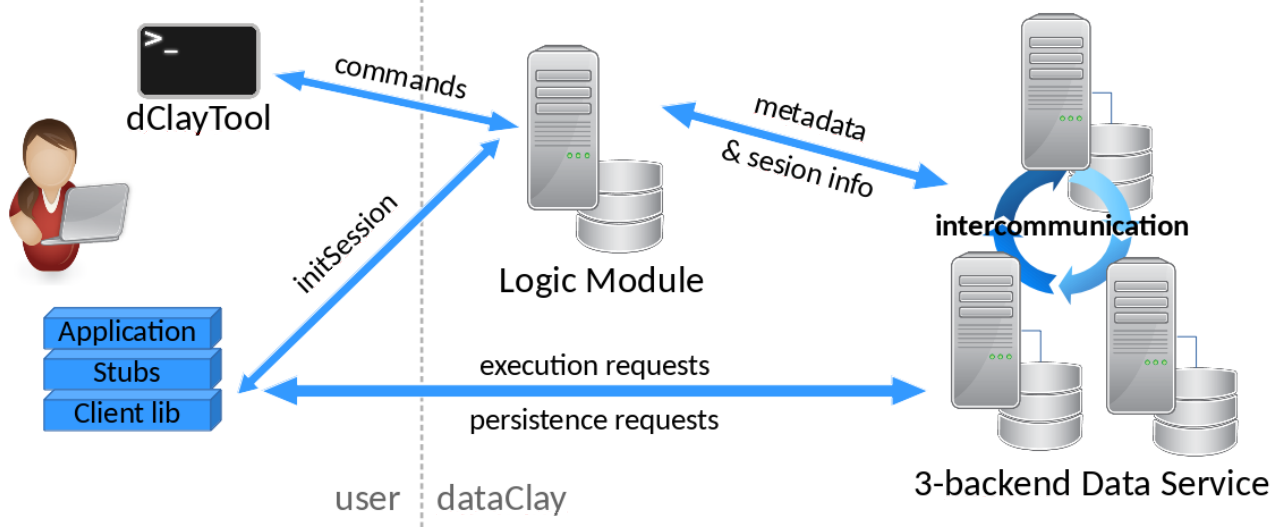
\includegraphics[scale=0.4]{Installation/dataClayOverview}
\caption{dataClay overview}
\label{fig:dataClayOverview}
\end{figure}

\subsection{Logic Module}\index{logic module}
The Logic Module is a unique centralized component that keeps track of every object metadata such as: its unique identifier, (replica) locations, and the dataset it is associated with. 

In addition, the Logic Module is in charge of management info, comprising: accounting, namespaces and datasets, permissions (contracts) and registered class models. That is, the information that can be registered in the system using the \textit{dClayTool} as shown in section \ref{sec:dClayTool}.

Furthermore, the Logic Module is the entry point for any user application, which must authenticate in the system to create a working session and gain permission to interact with the components of the Data Service.

\subsection{Data Service}\index{data service}\index{backend}
\label{sec:DataService}
The Data Service is deployed as a set of multiple backends. Any of these backends handles a subset of objects as well as the execution requests aiming to them. This means that every backend has an \textit{Execution Environment} for all supported languages (currently Java and Python) and an associated \textit{Storage System} to handle object persistence. In the case of Python, where multi-threading cannot be managed as Java does, it is possible to deploy multiple \textit{Execution Environments} sharing a single \textit{Storage System} thus enabling applications to exploit parallelism.

In order to enable \textit{Execution Environments} to handle any kind of object and execution request, the Logic Module is in charge to deploy registered classes to every Data Service backend. In this way, every backend can load stored objects as class instances and execute class methods on them corresponding to upcoming execution requests.

This means that when an application initializes a session with dataClay, it first establishes a connection with the Logic Module and obtains information about the available Data Service backends. At this point, the application is enabled to interact with the Data Service backends through stub classes (retrieved with the \textit{dClayTool}, section \ref{sec:dClayTool}) by submitting execution requests directly to them.



\section{Deployment with containers \index{docker}}

Keeping in mind the dataClay architecture, hereafter we show how to deploy a dataClay installation based on Docker \footnote{\url{https://www.docker.com}} containers.

A container image is a lightweight, stand-alone, executable package of a piece of software that includes everything needed to run it: code, runtime, system tools, system libraries, settings. 

In this way, we populate different Docker images corresponding to the main components of the dataClay architecture: the Logic Module and the Data Service. The latter actually comprises one image for each supported language since the corresponding execution requests are handled by separated containers (one per language). 

In order to retrieve these images and orchestrate dataClay services properly, following sections show different scenarios based on the standard \textit{docker-compose}\index{docker-compose} \footnote{\url{https://docs.docker.com/compose/}} tools.

\subsection{Single node installation}
\label{sec:SingleNodeInstall}
This first dataClay installation assumes that all services will run locally on a single node (e.g. your own laptop).

To this end, we will guide you through the installation process by looking at the details of the following \textit{docker-compose} YAML definition:

\begin{tBox}
 \begin{lstlisting}[language=docker-compose-2, frame=none]
version: '3.4'
services:
  logicmodule:
    image: "bscdataclay/logicmodule:2.0"
    ports:
      - "11034:11034"
    environment:
      - LOGICMODULE_PORT_TCP=11034
      - LOGICMODULE_HOST=logicmodule
      - DATACLAY_ADMIN_USER=admin
      - DATACLAY_ADMIN_PASSWORD=admin
    volumes:
      - ./prop/global.properties:/usr/src/dataclay/javaclay/cfgfiles/global.properties:ro
      - ./prop/log4j2.xml:/usr/src/dataclay/javaclay/log4j2.xml:ro
    healthcheck:
       interval: 5s
       retries: 10
       test: ["CMD-SHELL", "/usr/src/dataclay/javaclay/health_check.sh"]
         
  dsjava:
    image: "bscdataclay/dsjava:2.0"
    ports:
      - "2127:2127"
    depends_on:
      - logicmodule
    environment:
      - DATASERVICE_NAME=DS1
      - DATASERVICE_JAVA_PORT_TCP=2127
      - LOGICMODULE_PORT_TCP=11034
      - LOGICMODULE_HOST=logicmodule
    volumes:
      - ./prop/global.properties:/usr/src/dataclay/javaclay/cfgfiles/global.properties:ro
      - ./prop/log4j2.xml:/usr/src/dataclay/javaclay/log4j2.xml:ro
    healthcheck:
       interval: 5s
       retries: 10
       test: ["CMD-SHELL", "/usr/src/dataclay/javaclay/health_check.sh"]
       
  dspython:
    image: "bscdataclay/dspython:2.0"
    ports:
      - "6867:6867"
    depends_on:
      - logicmodule
      - dsjava
    environment:
      - DATASERVICE_NAME=DS1
      - LOGICMODULE_PORT_TCP=11034
      - LOGICMODULE_HOST=logicmodule
      - DATASERVICE_PYTHON_PORT_TCP=6867
    volumes:
      - ./prop/global.properties:/usr/src/dataclay/pyclay/cfgfiles/global.properties:ro
    healthcheck:
       interval: 5s
       retries: 10
       test: ["CMD-SHELL", "/usr/src/dataclay/pyclay/health_check.sh"]
 \end{lstlisting}
\end{tBox}

Before starting, the first step is to download the required images executing the following command from the directory where this \textit{docker-compose} file resides:
\begin{tBox}
 \begin{bash}
  > docker-compose pull
 \end{bash}
\end{tBox}

At this point, following subsections detail the different parts of the file and which ones can be customized.

\subsubsection{Logic Module}
The \textit{logicmodule}  service corresponds to the Logic Module. It is possible to customize the default Logic Module port, which is currently set to 11034 through environment variable \texttt{LOGICMODULE\_PORT\_TCP} and is mapped to host in \texttt{ports: - ``11034:11034''}. 

In this way, the Logic Module will publish its service at: \texttt{localhost:11034}. In section \ref{sec:ClientConfigFiles} it is described how to define the proper configuration files for user's applications considering this info.

\subsubsection{Data Service Backend - Java}
The \textit{dsjava}  service corresponds to the Java container of the Data Service Backend. Every Data Service backend is tagged with a name so containers for all supported languages can be defined as part of the same backend. This is specially useful to, for instance, define a unique database shared by different execution environments. In this case, the Java container is configured to be part of the Data Service backend called \textit{DS1} as defined via the \texttt{DATASERVICE\_NAME} variable. Furthermore, it is also necessary to specify the port that will be used to handle Java execution requests: \texttt{DATASERVICE\_JAVA\_PORT\_TCP=2127}.

Finally, we also need to specify the address of the Logic Module to enable this Java container to populate its service. To this end, we use the same variables and values as in the Logic Module service (\textit{logicmodule}): \texttt{LOGICMODULE\_HOST=logicmodule} and \texttt{LOGICMODULE\_PORT\_TCP=11034}.

\subsubsection{Data Service Backend - Python}
For Python, we only need to attach the container to a Data Service backend with Java support. In this case, we attach the Python container to \textit{DS1} Data Service backend through the \texttt{DATASERVICE\_NAME} variable. Furthermore, it is also necessary to specify the port that will be used to handle Java execution requests: \texttt{DATASERVICE\_PYTHON\_PORT\_TCP=6867}.

Finally, we also need to specify the address of the Logic Module to enable this Python container to populate its service. To this end, we use the same variables and values as in the Logic Module service (\textit{logicmodule}): \texttt{LOGICMODULE\_HOST=logicmodule} and \texttt{LOGICMODULE\_PORT\_TCP=11034}.

\subsection{Cluster installation}

If you want to deploy dataClay on a cluster of N nodes, you can create different \textit{docker-compose} files for each node depending on the setup you want.

In this section we describe a setup for a 3 node cluster with 1 node for the Logic Module and 2 nodes for Data Service backends. You can easy extrapolate this scenario to more complex ones, but always keeping in mind the following considerations/constraints for the current version of dataClay:

\begin{enumerate}
 \item The Logic Module is unique in the system. This means that only one of the nodes should have a docker-compose file with the Logic Module section.
 \item In this case, all services must be exposed using ``host'' network mode in order to make them visible and discoverable between different nodes and from the client application.
\end{enumerate}

\subsubsection{Node 1 - Logic Module}

The docker-compose file for the first node defining the Logic Module. Notice that using host network we do not need to map its port.

\begin{tBox}
 \begin{lstlisting}[language=docker-compose-2, frame=none]
version: '3.4'
services:
  logicmodule:
    image: "bscdataclay/logicmodule:2.0"
    ports:
      - "11034:11034"
    environment:
      - LOGICMODULE_PORT_TCP=11034
      - LOGICMODULE_HOST=logicmodule
      - DATACLAY_ADMIN_USER=admin
      - DATACLAY_ADMIN_PASSWORD=admin
    volumes:
      - ./prop/global.properties:/usr/src/dataclay/javaclay/cfgfiles/global.properties:ro
      - ./prop/log4j2.xml:/usr/src/dataclay/javaclay/log4j2.xml:ro
    healthcheck:
       interval: 5s
       retries: 10
       test: ["CMD-SHELL", "/usr/src/dataclay/javaclay/health_check.sh"]
 \end{lstlisting}
\end{tBox}

\subsubsection{Node 2 - Backend 1}

This node runs the Data Service backend \textit{DS1}, as specified through the \texttt{DATASERVICE\_NAME} variable.

Notice that the only variable that needs to be manually defined is \texttt{LOGICMODULE\_HOST}, which will be the host name of Node 1 where the Logic Module is deployed.

\begin{tBox}
 \begin{lstlisting}[language=docker-compose-2, frame=none]
version: '3.4'
services:
 dsjava:
    image: "bscdataclay/dsjava:2.0"
    ports:
      - "2127:2127"
    depends_on:
      - logicmodule
    environment:
      - DATASERVICE_NAME=DS1
      - DATASERVICE_JAVA_PORT_TCP=2127
      - LOGICMODULE_PORT_TCP=11034
      - LOGICMODULE_HOST=logicmodule
    volumes:
      - ./prop/global.properties:/usr/src/dataclay/javaclay/cfgfiles/global.properties:ro
      - ./prop/log4j2.xml:/usr/src/dataclay/javaclay/log4j2.xml:ro
    healthcheck:
       interval: 5s
       retries: 10
       test: ["CMD-SHELL", "/usr/src/dataclay/javaclay/health_check.sh"]
       
  dspython:
    image: "bscdataclay/dspython:2.0"
    ports:
      - "6867:6867"
    depends_on:
      - logicmodule
      - dsjava
    environment:
      - DATASERVICE_NAME=DS1
      - LOGICMODULE_PORT_TCP=11034
      - LOGICMODULE_HOST=logicmodule
      - DATASERVICE_PYTHON_PORT_TCP=6867
    volumes:
      - ./prop/global.properties:/usr/src/dataclay/pyclay/cfgfiles/global.properties:ro
    healthcheck:
       interval: 5s
       retries: 10
       test: ["CMD-SHELL", "/usr/src/dataclay/pyclay/health_check.sh"]
 \end{lstlisting}
\end{tBox}

\subsubsection{Node 3 - Backend 2}

Analogously to Node 2, this node runs the Data Service backend \textit{DS2}, as specified through the \texttt{DATASERVICE\_NAME} variable.

Finally, the only variable that needs to be manually defined is \texttt{LOGICMODULE\_HOST} with the host name of the Node 1 where Logic Module is deployed.

\begin{tBox}
 \begin{lstlisting}[language=docker-compose-2, frame=none]
version: '3.4'
services:
 dsjava2:
    image: "bscdataclay/dsjava:2.0"
    ports:
      - "2128:2128"
    depends_on:
      - logicmodule
    environment:
      - DATASERVICE_NAME=DS2
      - DATASERVICE_JAVA_PORT_TCP=2128
      - LOGICMODULE_PORT_TCP=11034
      - LOGICMODULE_HOST=logicmodule
    volumes:
      - ./prop/global.properties:/usr/src/dataclay/javaclay/cfgfiles/global.properties:ro
      - ./prop/log4j2.xml:/usr/src/dataclay/javaclay/log4j2.xml:ro
    healthcheck:
       interval: 5s
       retries: 10
       test: ["CMD-SHELL", "/usr/src/dataclay/javaclay/health_check.sh"]
       
  dspython2:
    image: "bscdataclay/dspython:2.0"
    ports:
      - "6868:6868"
    depends_on:
      - logicmodule
      - dsjava
    environment:
      - DATASERVICE_NAME=DS2
      - LOGICMODULE_PORT_TCP=11034
      - LOGICMODULE_HOST=logicmodule
      - DATASERVICE_PYTHON_PORT_TCP=6868
    volumes:
      - ./prop/global.properties:/usr/src/dataclay/pyclay/cfgfiles/global.properties:ro
    healthcheck:
       interval: 5s
       retries: 10
       test: ["CMD-SHELL", "/usr/src/dataclay/pyclay/health_check.sh"]
 \end{lstlisting}
\end{tBox}


\subsection{Enabling Python parallelism}
\label{sec:PythonParallelism}

In Section~\ref{sec:PythonConsiderationsExecutionEnvironment} we explain that the implementation details of the CPython Global Interpreter Lock forces that only one thread can execute Python code at once. However, and as introduced in Section~\ref{sec:DataService}, we can mitigate this problem by configuring dataClay to deploy multiple Python execution environments (backends) on a single node. The example below shows two Python execution environments that will load/store objects from the same Data Service \textit{DS1} ((\textit{dspython1, dspython2}).

\begin{tBox}
 \begin{lstlisting}[language=docker-compose-2, frame=none]
version: '3.4'
services:
  logicmodule:
    image: "bscdataclay/logicmodule:2.0"
    ports:
      - "11034:11034"
    environment:
      - LOGICMODULE_PORT_TCP=11034
      - LOGICMODULE_HOST=logicmodule
      - DATACLAY_ADMIN_USER=admin
      - DATACLAY_ADMIN_PASSWORD=admin
    volumes:
      - ./prop/global.properties:/usr/src/dataclay/javaclay/cfgfiles/global.properties:ro
      - ./prop/log4j2.xml:/usr/src/dataclay/javaclay/log4j2.xml:ro
    healthcheck:
       interval: 5s
       retries: 10
       test: ["CMD-SHELL", "/usr/src/dataclay/javaclay/health_check.sh"]
         
  dsjava:
    image: "bscdataclay/dsjava:2.0"
    ports:
      - "2127:2127"
    depends_on:
      - logicmodule
    environment:
      - DATASERVICE_NAME=DS1
      - DATASERVICE_JAVA_PORT_TCP=2127
      - LOGICMODULE_PORT_TCP=11034
      - LOGICMODULE_HOST=logicmodule
    volumes:
      - ./prop/global.properties:/usr/src/dataclay/javaclay/cfgfiles/global.properties:ro
      - ./prop/log4j2.xml:/usr/src/dataclay/javaclay/log4j2.xml:ro
    healthcheck:
       interval: 5s
       retries: 10
       test: ["CMD-SHELL", "/usr/src/dataclay/javaclay/health_check.sh"]
       
  dspython:
    image: "bscdataclay/dspython:2.0"
    ports:
      - "6867:6867"
    depends_on:
      - logicmodule
      - dsjava
    environment:
      - DATASERVICE_NAME=DS1
      - LOGICMODULE_PORT_TCP=11034
      - LOGICMODULE_HOST=logicmodule
      - DATASERVICE_PYTHON_PORT_TCP=6867
    volumes:
      - ./prop/global.properties:/usr/src/dataclay/pyclay/cfgfiles/global.properties:ro
    healthcheck:
       interval: 5s
       retries: 10
       test: ["CMD-SHELL", "/usr/src/dataclay/pyclay/health_check.sh"]
       
  dspython2:
    image: "bscdataclay/dspython:2.0"
    ports:
      - "6868:6868"
    depends_on:
      - logicmodule
      - dsjava
    environment:
      - DATASERVICE_NAME=DS1
      - LOGICMODULE_PORT_TCP=11034
      - LOGICMODULE_HOST=logicmodule
      - DATASERVICE_PYTHON_PORT_TCP=6868
    volumes:
      - ./prop/global.properties:/usr/src/dataclay/pyclay/cfgfiles/global.properties:ro
    healthcheck:
       interval: 5s
       retries: 10
       test: ["CMD-SHELL", "/usr/src/dataclay/pyclay/health_check.sh"]
       
 \end{lstlisting}
\end{tBox}

At this point, check Session~\ref{sec:FullTestOtherExamples} if you want to get introduced on how to exploit parallelism with this kind of configurations.


\subsection{Tuning dataClay}

dataClay allows to tune some specific settings (detailed in next sections) using a property file located on a specific path. 

In the application/client side the default path of this file is \texttt{./cfgfiles/global.properties} and can be also defined via the environment variable \texttt{DATACLAY\_GLOBAL\_CONFIG}.

In the server-side the default path is the same, but following previous examples with Docker containers we must define a \textit{volume} to load it. Given the first docker-compose file for a local installation, and assuming that there is a property file located at \texttt{./cfgfiles/global.properties} (relative to the docker-compose file), the volume can be mounted in a per-service basis as illustrated below:

\begin{tBox}
 \begin{lstlisting}[language=docker-compose-2, frame=none]
version: '3.4'
services:
  logicmodule:
    image: "bscdataclay/logicmodule:2.0"
    ports:
      - "11034:11034"
    environment:
      - LOGICMODULE_PORT_TCP=11034
      - LOGICMODULE_HOST=logicmodule
      - DATACLAY_ADMIN_USER=admin
      - DATACLAY_ADMIN_PASSWORD=admin
    volumes:
      - ./prop/global.properties:/usr/src/dataclay/javaclay/cfgfiles/global.properties:ro
      - ./prop/log4j2.xml:/usr/src/dataclay/javaclay/log4j2.xml:ro
    healthcheck:
       interval: 5s
       retries: 10
       test: ["CMD-SHELL", "/usr/src/dataclay/javaclay/health_check.sh"]
         
  dsjava:
    image: "bscdataclay/dsjava:2.0"
    ports:
      - "2127:2127"
    depends_on:
      - logicmodule
    environment:
      - DATASERVICE_NAME=DS1
      - DATASERVICE_JAVA_PORT_TCP=2127
      - LOGICMODULE_PORT_TCP=11034
      - LOGICMODULE_HOST=logicmodule
    volumes:
      - ./prop/global.properties:/usr/src/dataclay/javaclay/cfgfiles/global.properties:ro
      - ./prop/log4j2.xml:/usr/src/dataclay/javaclay/log4j2.xml:ro
    healthcheck:
       interval: 5s
       retries: 10
       test: ["CMD-SHELL", "/usr/src/dataclay/javaclay/health_check.sh"]
       
  dspython:
    image: "bscdataclay/dspython:2.0"
    ports:
      - "6867:6867"
    depends_on:
      - logicmodule
      - dsjava
    environment:
      - DATASERVICE_NAME=DS1
      - LOGICMODULE_PORT_TCP=11034
      - LOGICMODULE_HOST=logicmodule
      - DATASERVICE_PYTHON_PORT_TCP=6867
    volumes:
      - ./prop/global.properties:/usr/src/dataclay/pyclay/cfgfiles/global.properties:ro
    healthcheck:
       interval: 5s
       retries: 10
       test: ["CMD-SHELL", "/usr/src/dataclay/pyclay/health_check.sh"]
 \end{lstlisting}
\end{tBox}

\subsection{Singularity}
dataClay can also be deployed using Singularity: once converted the Docker images as explained in the \href{https://sylabs.io/guides/3.0/user-guide/build_a_container.html#downloading-an-existing-container-from-docker-hub}{Singularity official guide}, each container can be orchestrated by using \href{https://singularityhub.github.io/singularity-compose}{Singularity Compose} (e.g. by manually porting the configurations contained in docker-compose.yml example files).

\subsection{Memory Management and Garbage Collection}\index{memory management}\index{garbage collection}

In section \ref{sec:GarbageCollection} we have introduced that dataClay runs some processes to keep memory and disk usage in a healthy state. On the one hand, flushing objects from memory to disk when memory usage reaches a certain threshold. On the other hand, keeping track of reference counters to detect objects that are no longer accessible so they can be removed from the system.

To control the impact of these processes on the system performance, dataClay provides the administrator with the capability to configure the following parameters via \textit{global.properties} file. Notice that time parameters are always expressed in milliseconds.

\begin{table}[H]
\footnotesize
\begin{tBox}
\centering
\begin{tabular}{p{57mm} | p{27mm} |  >{\raggedright\arraybackslash}p{50mm}}
\textbf{property} & \textbf{default value} & \textbf{description} \\
\hline
\verb MEMMGMT_PRESSURE_FRACTION & 0.7 (70\%) & Fraction of memory usage from which to consider that it is under pressure. \\
\hline
\verb MEMMGMT_CHECK_TIME_INTERVAL & 5000 (5 seconds) & Periodicity to check memory usage. \\
\hline
\verb GLOBALGC_CHECK_TIME_INTERVAL & 86400000 (1 day) & Periodicity to check and collect objects from underlying storage. \\
\end{tabular}
\label{table:GarbageCollection}
\end{tBox}
\end{table}

An example of the \textit{global.properties} file with non-default values would be as follows:

\begin{tBox}
 \begin{bash}
MEMMGMT_PRESSURE_FRACTION=0.8
MEMMGMT_CHECK_TIME_INTERVAL=8000
GLOBALGC_CHECK_TIME_INTERVAL=1000000
 \end{bash}
\end{tBox}

\PREFETCH{
\subsubsubsection{Data Prefetching}\index{prefetching}
\label{sec:prefetchingTuning}
As explained in Section \ref{sec:prefetching}, the user can activate data prefetching in dataClay in order to improve the application performance. In order to do so, the following property should be set to true in the \textit{global.properties} file of both the logic module and data services when dataClay is installed.

\begin{table}[H]
\footnotesize
\begin{tBox}
\centering
\begin{tabular}{p{57mm} | p{27mm} |  >{\raggedright\arraybackslash}p{50mm}}
\textbf{property} & \textbf{default value} & \textbf{description} \\
\hline
\verb PREFETCHING_ENABLED & FALSE & Activate or deactivate prefetching in dataClay. \\
\end{tabular}
\label{table:GarbageCollection}
\end{tBox}
\end{table}

Keep in mind that prefetching should also be activated when registering an application using dataClay tool, as explained in Section \ref{sec:newModel}.
}
  \chapterimage{Client.jpg} % Chapter heading image

\chapter{Client configuration}

\section{Client libraries}
\label{sec:ClientLibraries}

In order to connect your applications with dataClay services you need a client library for your preferred programming language.

If you are developing a Java application you can obtain the library following instructions in \ref{sec:FullDemo} (downloading our zip file as exposed in Section~\ref{sec:DownloadZIP} or following instructions for POM-based projects in Section~\ref{sec:POMbasedProjects}).

In case you are developing a Python application, you can easily install the Python module with \textit{pip} command:

\begin{tBox}
\begin{bash}
> pip install dataClay
\end{bash}
\end{tBox}

\section{Configuration files}
\label{sec:ClientConfigFiles}

The basic client configuration for an application is the minimum information required to initialize a session with dataClay. To this end two different files are required: the \textit{session.properties}\index{session.properties} file and the \textit{client.properties}\index{client.properties} file.

\subsection{Session properties}
This file contains the basic info to initialize a session with dataClay. It is automatically loaded during the initialization process (\texttt{DataClay.init()}\index{DataClay.init()} in Java or \texttt{api.init()}\index{api.init()} in Python) and its default path is \texttt{./cfgfiles/session.properties}. This path can be overridden by setting a different path through the environment variable \texttt{DATACLAYSESSIONCONFIG}. 

Here is an example:

\begin{tBox}
 \begin{bash}
  Account=MyAccount
  Password=MyPassword
  StubsClasspath=/home/me/myapp/stubs
  DataSetForStore=MyDataset
  DataSets=MyDataset,OtherDataSet
  LocalBackend=DS1
 % DataClayClientConfig=/home/me/myapp/client.properties
 \end{bash}
\end{tBox}

\texttt{Account} and \texttt{Password} properties are used to specify user's credentials. 

\texttt{StubsClasspath} defines a path where the stub classes can be located. That is, the path where \textit{dClayTool} (exposed in section \ref{sec:dClayTool}) saved our stub classes after calling \texttt{GetStubs} operation.

\texttt{DataSetForStore} specifies which dataset the application will use in case a \textit{makePersistent} request is produced to store a new object in the system, and \texttt{DataSets} provide information about the datasets the application will access (normally it includes the \texttt{DataSetForStore}). 

\texttt{LocalBackend} defines the default backend that the application will access when using either \texttt{DataClay.LOCAL} in Java or \texttt{api.LOCAL} in Python (examples of this can be found in API sections \ref{sec:JavaAPI} and \ref{sec:PythonAPI}). 

%Finally, the \texttt{DataClayClientConfig} contains a path pointing to \textit{client.properties} file, which is the second file required as exposed in next section.

\subsection{Client properties}
This file contains the minimum service info to connect applications with dataClay. It is also loaded automatically during the initialization process and its default path is \texttt{./cfgfiles/client.properties}, which can be overriden by setting the environment variable \texttt{DATACLAYCLIENTCONFIG}.

Here is an example:

\begin{tBox}
 \begin{bash}
 HOST=localhost
 TCPPORT=11034
 \end{bash}
\end{tBox}

As you can see, it only requires two properties to be defined: \texttt{HOST} and \texttt{TCPPORT}; comprising the full address to be resolved in order to initialize a session with dataClay from your application.


\part{Bibliography and index}

%----------------------------------------------------------------------------------------
%	BIBLIOGRAPHY
%----------------------------------------------------------------------------------------
\chapterimage{TOC.jpg}
\chapter*{Bibliography}
\addcontentsline{toc}{chapter}{\textcolor{basecolor}{Bibliography}}

%------------------------------------------------

%\section*{Articles}
%\addcontentsline{toc}{section}{Articles}
%\printbibliography[heading=bibempty,type=article]

%------------------------------------------------

%\section*{Books and Ph.D. Thesis}
%\addcontentsline{toc}{section}{Books}
\printbibliography[heading=bibempty]

%----------------------------------------------------------------------------------------
%	INDEX
%----------------------------------------------------------------------------------------

\cleardoublepage
\phantomsection
\setlength{\columnsep}{0.75cm}
\addcontentsline{toc}{chapter}{\textcolor{basecolor}{Index}}
\printindex

%----------------------------------------------------------------------------------------

\end{document}
